\documentclass[a4paper,12pt]{jsarticle}

% 数式
\usepackage{siunitx} % SI単位系表示
\usepackage{amsmath,amsfonts}
\numberwithin{equation}{subsection} % section.subsection.式番号 / section.式番号なら{equation}{section}
\usepackage{bm}
\usepackage{color}
\usepackage[version=4]{mhchem} % graphicx 使用中にこれを使うとdvipdfmxを使ってても BoundingBox 情報のない画像ファイルだと BoundingBox を生成できなくなるので、手動設定かEPS変換が必要

% ルビ
\usepackage{pxrubrica}
% 文章を囲む
\usepackage{ascmac}
% 複数行コメントアウト(\if0と\fiで囲むやつはパッケージなしで可能)
\usepackage{comment}
% 箇条書き機能拡張(・非表示など)
\usepackage{enumitem}
% 表
\usepackage{multirow} % 縦方向セル結合
\usepackage{threeparttable} % 表に脚注追加
\usepackage{longtable} % 長い表
\usepackage{array} % 表を中央揃えにして幅指定
\newcolumntype{C}[1]{>{\hfil}m{#1}<{\hfil}}

% 画像
\usepackage[dvipdfmx]{graphicx}
\usepackage{caption} % 図キャプション設定パッケージ

\renewcommand{\figurename}{Fig} % 図からFig.に変更
\renewcommand{\tablename}{Table} % 図からTable.に変更

\numberwithin{figure}{subsection} % section.subsection.図番号 / section.図番号なら{figure}{section}

\usepackage{subfig} % 図を並べる
\usepackage[subrefformat=parens]{subcaption}

% 参考文献関係
\usepackage[sorting=none, refsegment=section]{biblatex} % 本文中での参照順:sorting=none, 章/節ごとにリスト表示:refsegment=section
\addbibresource{zemi.bib} % 参考文献ファイルのリスト(.bibファイル)を指定

% BiBTeX関連
\usepackage{url}

% 行番号を表示する。添削時のみに使い、事務提出版ではコメントアウトする
%\usepackage{lineno}
%\linenumbers

% hyperref パッケージは,かなり多くのコマンドを再定義するため,できるだけ後ろの方で読み込むように
% PDF 内で外部リンクや文書内リンクを生成したい場合に使う(好みによる)
% 印刷時に色が出るかどうかは、使用する PDF viewer の挙動による。
% 紙媒体で修論を提出する場合、文字色は黒にするのが適切なので要注意。
\usepackage[dvipdfmx,colorlinks=true,allcolors=blue]{hyperref}
%\usepackage[hidelinks]{hyperref}
% PDF 内のしおりの文字化けを防ぐ
% 先頭に \RequirePackage{plautopatch} を追加すれば 2020 年以降の TeX 環境では不要
\usepackage{pxjahyper} % (u)pLaTeXのときのみかく

% 問題番号設定
\newcounter{toinum}
\newcommand{\toi}{
  \refstepcounter{toinum}
  \noindent\textbf{問題\thesection.\thetoinum.}\par
}
\newcounter{subtoinum}[toinum]
\newcommand{\subtoi}{
  \refstepcounter{subtoinum}
  \noindent\textbf{(\thesubtoinum) }
}




\begin{document}

\begin{center}
  \Large
  松山研全体ゼミ勉強会 原子炉物理 座学
  \normalsize
\end{center}


\section{序論}
\subsection{原子炉/原子炉物理とは何か}
\begin{itembox}[l]{「原子炉物理」の定義}
  原子炉物理(Reactor Physics)とは、原子炉内で生じる\emph{中性子の挙動と原子核の反応を予測}する学問である。
\end{itembox}
\vskip\baselineskip
言葉の定義にあるように、原子炉の物理現象(Physics of Reactor)全てを取り扱うのではなく、核分裂反応を中核とする
中性子と原子核の相互作用に焦点をあてた学問である。しかしながら、中性子と原子核の相互作用の確率は原子炉の体系
に依存するため、他の物理現象の影響(例:温度、物質組成の変化)を受ける。したがって、最終的には様々な物理現象を考慮
する必要がある。
\begin{comment}
  BWRの核と熱水力の結合の例などを挙げる
\end{comment}

\vskip3\baselineskip
では、そもそも原子炉とは何であろうか。核燃料物質、核原料物質、原子炉及び放射線の定義に関する政令では
次のような定義を用いている。
\vskip\baselineskip
\begin{itembox}[l]{「原子炉」の定義}
  \emph{核燃料}を用い、\emph{制御可能な核分裂の連鎖反応}を\emph{中性子源無しに持続}できる装置、
  または持続する恐れのある装置以外のもの\\
  「核燃料物質、核原料物質、原子炉及び放射線の定義に関する政令」より要約
\end{itembox}
\vskip\baselineskip

核分裂反応は、重い原子核が2つに分裂し複数の中性子を放出する反応である。核分裂反応は主に中性子が原子核に吸収される
ことで発生するため、核分裂で発生した中性子(\emph{核分裂中性子})で核分裂反応を再び引き起こすことができる。
これが\emph{連鎖反応}と呼ばれる所以である。もし、核分裂中性子のみで一定の核分裂反応速度を維持できるなら、
中性子源無しに核分裂連鎖反応を持続させられる。これが原子炉の「\emph{臨界}」である。また、核分裂反応速度
が増加していく状態を\emph{超臨界}と呼ぶ。逆に核分裂反応が収束していく状態を\emph{未臨界}と呼ぶ。
原子炉には、体系の臨界性を変化させ核分裂連鎖反応を制御することが求められる。

\subsection{原子炉の利益}
原子炉には様々な用途が存在する。その用途は次のように大別できる。
\begin{itemize}
  \item 核反応による\emph{エネルギーの利用}
  \item 効率的な\emph{中性子源としての利用}(放射線利用)
\end{itemize}

1つ目は核分裂反応で発生したエネルギーを熱として取り出し利用することである。現在最も盛んなエネルギー利用法
は\emph{発電}である。原子力発電所では核エネルギーを用いて冷却材(主に水)を加熱し、蒸気タービンを回して発電する。
また、将来的にはより冷却材温度の高い高温ガス炉により、高熱を利用した\emph{水素製造}や\emph{製鉄}を行うことも期待されている。

現状主力となっている発電方法は、化石燃料の燃焼時の熱エネルギーを利用した火力発電であるが、温室効果ガス排出や
資源が地理的に偏在していること、燃料費が高く変動性もあることが課題となっている。また、水素製造や製鉄においても
化石燃料を用いることが課題となっている。例えば現在主流の水素製造法であるメタン水蒸気改質法の化学反応式は
\begin{equation}
  \ce{\textcolor{red}{\textbf{CH4}} + 2H2O -> \textcolor{red}{\textbf{CO2}} + 4H2}
\end{equation}
であり、天然ガス由来のメタンを消費し、二酸化炭素を排出することが欠点となっている。
製鉄については、高炉で鉄鉱石から銑鉄を得る際の正味の化学反応式は
\begin{equation}
  \ce{Fe2O3 + \textcolor{red}{\textbf{3CO}} -> 2Fe + \textcolor{red}{\textbf{3CO2}}}
\end{equation}
である。日本の場合、2023年度時点で二酸化炭素排出の1割強が製鉄由来であり、発電、道路輸送に次いで多い
二酸化炭素排出源となっている\cite{National-GHG-Inventory-Doc-Jpn-2025}。

原子炉をエネルギー源として利用すれば、これらの問題を解決することができる。
核分裂反応による温室効果ガス排出が無く、エネルギー密度が高いため少量の燃料を輸入するだけで
大量のエネルギー源を確保できる。天然ガスの主成分であるメタンの燃焼と、
主な核燃料であるウラン235の核分裂反応例の比較を次に示す。エネルギーの単位は
ウラン235、およびメタン分子1つあたりのエネルギー(メガ電子ボルト)、メタンの反応熱は
低位発熱量である。
\begin{align}
  \ce{^{235}U + n -> ^{92}Kr + ^{141}Ba + 3n} + \text{約} \textcolor{red}{\mathbf{200}} \  \text{[MeV/n]}\\
  \ce{CH4 + 2O2 -> CO2 + 2H2O} + \textcolor{red}{\mathbf{8.3 \times 10^{-6}}} \  \text{[MeV/n]}
\end{align}
発生するエネルギー核分裂反応はメタン燃焼の$2.4 \times 10^{7}$倍であり、エネルギー密度の差は歴然である。
これこそ原子炉のエネルギー利用の最大の利点である。

\vskip\baselineskip
\begin{shadebox}
  \toi 液化LNGガスと二酸化ウランペレットの\emph{質量に対する熱量}、\emph{体積当たりの熱量}を
  比較せよ。必要に応じて以下の値を使用すること。
  \begin{itemize}
    \item アボガドロ定数: $N_A = 6.022140857 \times 10^{23} \ \text{[mol$^{-1}$]}$
    \item 電子ボルトからジュールへの換算: $1.6021766208 \times 10^{-19} \ \text{[J/eV]}$
    \item 統一原子質量: $1.66053906892 \times 10^{-24} \ \text{[g/u]}$
    \item 二酸化ウラン(面心立方格子、蛍石型)\\
          単位格子あたりに酸素8つ、ウラン4つ 格子定数: $0.547 \ \text{[\si{\nm}]}$
    \item \ce{O2}原子量 $15.9994 \ \text{[u]}$
    \item \ce{^{235}U}、\ce{^{238}U}原子質量 それぞれ$ 235.0439 \ \text{[u]} $、$ 238.0508 \ \text{[u]} $
    \item \ce{^{235}U}核分裂あたりの平均エネルギー $ 202.5 \ \text{[\si{\MeV}]} $
    \item LNG発熱量 $ 54.6 \ \text{[\si{\mega\J/\kg}]} $
    \item LNG液密度 $ 0.460 \ \text{[\si{\kg/\L}]} $
  \end{itemize}
\end{shadebox}
\vskip\baselineskip

原子炉を用いれば、水素製造は高温の水蒸気\footnote{高温水蒸気電解法で\SI{700}{\degreeCelsius}、
熱化学法ISプロセスで\SI{900}{\degreeCelsius}}を用いて水から二酸化炭素排出無しで水素を製造できる。
正味の化学反応式は
\begin{equation}
  \ce{2H2O -> 2H2 + O2}
\end{equation}
である。この手法であれば、水以外の天然資源を使わず、かつ温室効果ガスを排出せずに
水素を製造できる。また、発生した水素を用いて水素還元製鉄と呼ばれる温室効果ガスを
排出しない製鉄も可能となる。
\begin{equation}
  \ce{Fe2O3 + 3H2 -> 2Fe + 3H2O}
\end{equation}
このように、電力以外の用途についても、原子炉は環境に良いエネルギー源として魅力的な存在である。

\vskip3\baselineskip

2つ目は、放射線源としての利用である。原子炉は中性子源無しに核分裂連鎖反応を維持できるため、加速器中性子源とは異なり
簡単かつ電力消費無しに大量の中性子を発生させることができる。中性子は核反応を用いて目的とする核種を製造したり、
減らしたい核種を他の核種に変換することができるため、原子炉中性子源は効率的な中性子源として利用されている。
主な核変換としては以下の例がある。
  \begin{itemize}
    \item 核燃料の増殖: \ce{ ^{238}U + n ->T[捕獲反応] ^{239}U ->T[$\beta^{-}$][23.45 min] ^{239}Np ->T[$\beta^{-}$][2.356 d] ^{239}Pu }
    \item 放射性同位体(Radioisotope; RI)製造: \ce{ ^{98}Mo + n -> ^{99}Mo ->T[$\beta^{-}$][2.749 d] ^{99m}Tc }
    \item 核廃棄物の核変換\\
          マイナーアクチノイド(\ce{U}、\ce{Pu}以外のアクチノイド): \[\ce{^{237}Np}\mbox{(半減期214万年)} \ce{ + n ->T[核分裂] ^{104}Tc + ^{130}Sn + 4n}\]
          \[\ce{^{104}Tc ->T[$\beta^{-}$][18.3 min] ^{104}Ru} \]
          \[\ce{^{130}Sn ->T[$\beta^{-}$][3.72 min] ^{130}Sb ->T[$\beta^{-}$][39.5 min] ^{130}Te} \mbox{(安定核)} \]
          長寿命核分裂生成物(LLFP:Long-lived fission products): \[\ce{^{129}I}\mbox{(半減期1570万年)} \ce{ + n -> ^{130}I ->T[$\beta^{-}$][12.36 h] ^{130}Xe} \mbox{(安定核)} \]
  \end{itemize} 
ウラン238から作られるプルトニウム239は、ウラン235と同じく核分裂を起こしやすい核種であり核燃料として利用できる。
この反応を使えば核燃料を燃やしながら核燃料物質を新たに製造でき、場合によっては消費量を超える量をも製造
できる可能性がある。このような燃料を増殖する原子炉を\emph{増殖炉}と呼ぶ。
核燃料以外の放射性同位体の製造としては、ここで挙げた医療用RIである\ce{^{99}Mo}/\ce{^{99m}Tc}を中心に
様々な核種の製造が期待されている。現在\ce{^{99}Mo}/\ce{^{99m}Tc}の製造は海外の原子炉のみであり、多くが
老朽化している上、半減期(半分の量が崩壊して他の核種になるのにかかる時間)が短いためテロや自然環境の
影響を受けやすい空輸で輸入せざるを得ない\cite{JRIA-MedRI-2021Nov}。
故に国内で製造できる原子炉を確保することが重要な課題となっている。
核廃棄物の核変換は、使用済み核燃料によって発生した廃棄物の長半減期の放射性同位体を
短半減期、安定核種に変換して処分の負担を軽減することが目的である。日本では、
放射性廃棄物を廃棄物・有用な物質に分離し、長寿命核種を変換する\emph{分離変換}が提案されており、
最終処分場の面積を最大$1/100$に抑え、1万年程度かかっていたウラン鉱石と同等の毒性に落ちるまでの
期間が300年まで短縮することができる。

核変換以外の放射線源としての用途としては、中性子ビームの利用がある。原子炉で発生した中性子を
ビームとして取り出し、物質の微細構造を分析したり、放射線透過による画像化、
ホウ素中性子捕獲療法によるがん治療を行うことができる。日本原子力研究開発機構の研究炉「JRR-3」は
中性子ビーム取り出し用の施設が備わっており、様々な研究に利用されている。



\subsection{核燃料}
主な核燃料物質としては\textbf{ウラン235}がある。ウランは鉱石や海水中に存在するため容易に
入手できる。しかしながら、ウラン235の天然存在比は0.72 at\%と少数であり、
それ以外のほぼ全ては核分裂を起こしにくいウラン238で占められている。故に天然存在比の
ウランでは原子炉を臨界にしにくい。故に、殆どの原子炉ではウラン235を\emph{濃縮}し
臨界しやすくして用いる。濃縮の度合いを\emph{濃縮度}と呼び、20 wt\%未満のものを\emph{低濃縮ウラン
(Low Enriched Uranium; LEU)}、それ以上のものを\emph{高濃縮ウラン(High Enriched Uranium; HEU)}
と呼ぶ。一方濃縮時に発生したウラン235が天然存在比未満のウランは減損ウランや\emph{劣化ウラン
(Depleted Uranium; DU)}と呼ばれる。一般的な商用炉の濃縮度は3~5 wt\%であり、LEUに分類される。
一方、研究炉や原子力艦船用原子炉\footnote{研究炉は小型炉心で大量の中性子を供給するために
高出力密度にする必要があることから、艦船用原子炉は船舶に搭載できるほど小型かつ長寿命にすることから、
それぞれHEUを必要とする}、核兵器\footnote{しばしば原子炉を制御できる理由は低濃縮度であるからという
説明がされるが誤りである。実際は原子炉が遅発臨界の領域で核反応を起こすからである。核兵器と一部の
特殊な研究炉のみ即発臨界を利用する。}などにはHEUを利用する。HEUは核兵器拡散リスクが高いため
商用炉では用いず、研究炉でも利用を最小限に抑える取り組みがなされている。なお、20\%を境界とするのは、
核兵器に必要な90\%付近までの濃縮に必要な分離作業の大半が20\%までの濃縮に費やされるためである。

近年では燃料交換の頻度を少なくするため、商用炉燃料の濃縮度を高くする潮流があり、
5~20 wt\%濃縮の高純度低濃縮ウラン(High-Assay Low Enriched Uranium; HALEU)
や5~10 wt\%濃縮の「LEU+」が次世代燃料として注目されている
\footnote{現状、国内生産の濃縮ウランは実質的に5\%の制約がある。これは濃縮度が5\%を超える場合、
「特定のウラン加工施設のための安全審査指針」の適用を受け、大幅な設備変更・投資が必要になって
しまうからである。なお、2025年現在で5\%を超える商用燃料は国外でも照射試験が開始されたばかり
である\cite{WNN-LEUplus-2025Apr}\cite{FEPC-LEUplus-2024Feb}。}。

他の核燃料としては\textbf{プルトニウム239}がある。この核種も核分裂を起こしやすく、
更に核分裂を起こしにくいウラン238から製造できるため、核燃料を燃やしながら増殖できる
\emph{増殖炉}を実現できる可能性がある。燃料の原料となるウラン238は、ウラン濃縮の過程で
廃品として発生する劣化ウランを用いれば良いので、ウラン資源の利用率を大幅に向上できるという
利点もある。日本が\emph{核燃料サイクル}の構築を目標としているのは、増殖炉を用いれば
資源の対外依存を抑えながら安定的にエネルギーを供給することができるからである。

% 章ごとの参考文献欄
\printbibliography[segment=\therefsegment,heading=subbibliography]

\newpage
\section{臨界、原子炉と核データ}

\subsection{中性子増倍率}
\label{subsec:multipilication_factor}
核分裂連鎖反応では、核分裂の反応数が指数関数的に増減する。
1つの中性子が核分裂を引き起こし、2つの中性子が放出される体系を考える。この2つの核分裂中性子がどちらも
次の核分裂を起こす場合、この体系の中性子増倍率$k$は次のようになる。
\begin{equation}
  k = \frac{\text{発生した核分裂中性子のうち核分裂を起こす数}}{\text{核分裂を起こした中性子数}} = \frac{2}{1} = 2
\end{equation}
実際には核分裂反応はバラバラなタイミングで起こるが、簡単のために「世代」という概念を導入して考える。
丁度アニメーションのフレームと同じで、バラバラなタイミングで起こる核分裂反応を、あるタイミングで一気に
発生するものとして考える。1フレームあたりの時間は、核分裂が発生してから次の核分裂が発生するまでの平均的な
時間を使う。この時間を\emph{即発中性子寿命}、または\emph{世代時間}と呼ぶ。
中性子増倍率はある世代の中性子数を一つ前の世代の中性子数で割ったものとしても定義される。
\begin{equation}
  \label{eq:multi_factor}
  k = \frac{\text{ある世代の中性子数}}{\text{一つ前の世代の中性子数}}
\end{equation}
この中性子増倍率$k$が1より大きい状態を\emph{超臨界}、1より小さい状態を\emph{未臨界}、1の状態を\emph{臨界}と呼ぶ。
\[
k \; \left\{
  \begin{array}{ll}
    > 1 & \text{超臨界} \\
    = 1 & \text{臨界} \\
    < 1 & \text{未臨界}
  \end{array}
\right.
\]

\subsection{中性子と原子核の反応}
中性子は電荷を持たないため原子核に近づきやすく、原子核と\SI{e-12}{\centi\metre}程度まで近づくと
原子核と相互作用する。この相互作用は、大きく散乱反応(scattering)と吸収反応(absorption)に分けられる。

\subsubsection{散乱反応}
散乱反応はさらに\emph{弾性散乱}(elastic scattering)と\emph{非弾性散乱}(inelastic scattering)の2つに分けられる。
弾性散乱では中性子と原子核の運動エネルギーは保存されるため、一般には中性子の運動エネルギーの一部が原子核(ターゲット核)
に移り中性子の運動方向とエネルギーが変化する。弾性散乱には、中性子が原子核に取り込まれずに原子核のポテンシャルで散乱される
ポテンシャル散乱と、中性子が一旦原子核に取り込まれ複合核となった後にエネルギーを失わずに放出される共鳴散乱がある。
非弾性散乱ではターゲット核に移ったエネルギーの一部が原子核の励起エネルギーに使われる。
そのため、非弾性散乱は中性子のエネルギーがターゲット核の最低の励起エネルギーよりも大きい場合にのみ起こる。
Fig.~\ref{fig:neutron_scattering}は、いくつかの核種の弾性散乱断面積を示している。黒鉛のように配列的に並ぶ材料に
対しては、低エネルギー中性子は回析を起こす(干渉性散乱)。また、水分子の水素原子のように、結合によって
自由に動き回れないことによる断面積の変化も見られる(非干渉性非弾性散乱)。
中エネルギー領域の中性子に対しては核力のポテンシャルによって散乱し、断面積は一定の値を示す。
高エネルギーの領域の中性子に対しては核力のポテンシャルを超えて原子核に取り込まれる部分が出てくる。

Fig.~\ref{fig:neutron_inelastic_scattering}は、\ce{^{238}U}と\ce{^{90}Zr}の非弾性散乱断面積、
Fig.~\ref{fig:neutron_inelastic_scattering_U238}は\ce{^{238}U}の励起準位を考慮した非弾性散乱断面積を示している。


\begin{figure}[htbp]
  \centering
  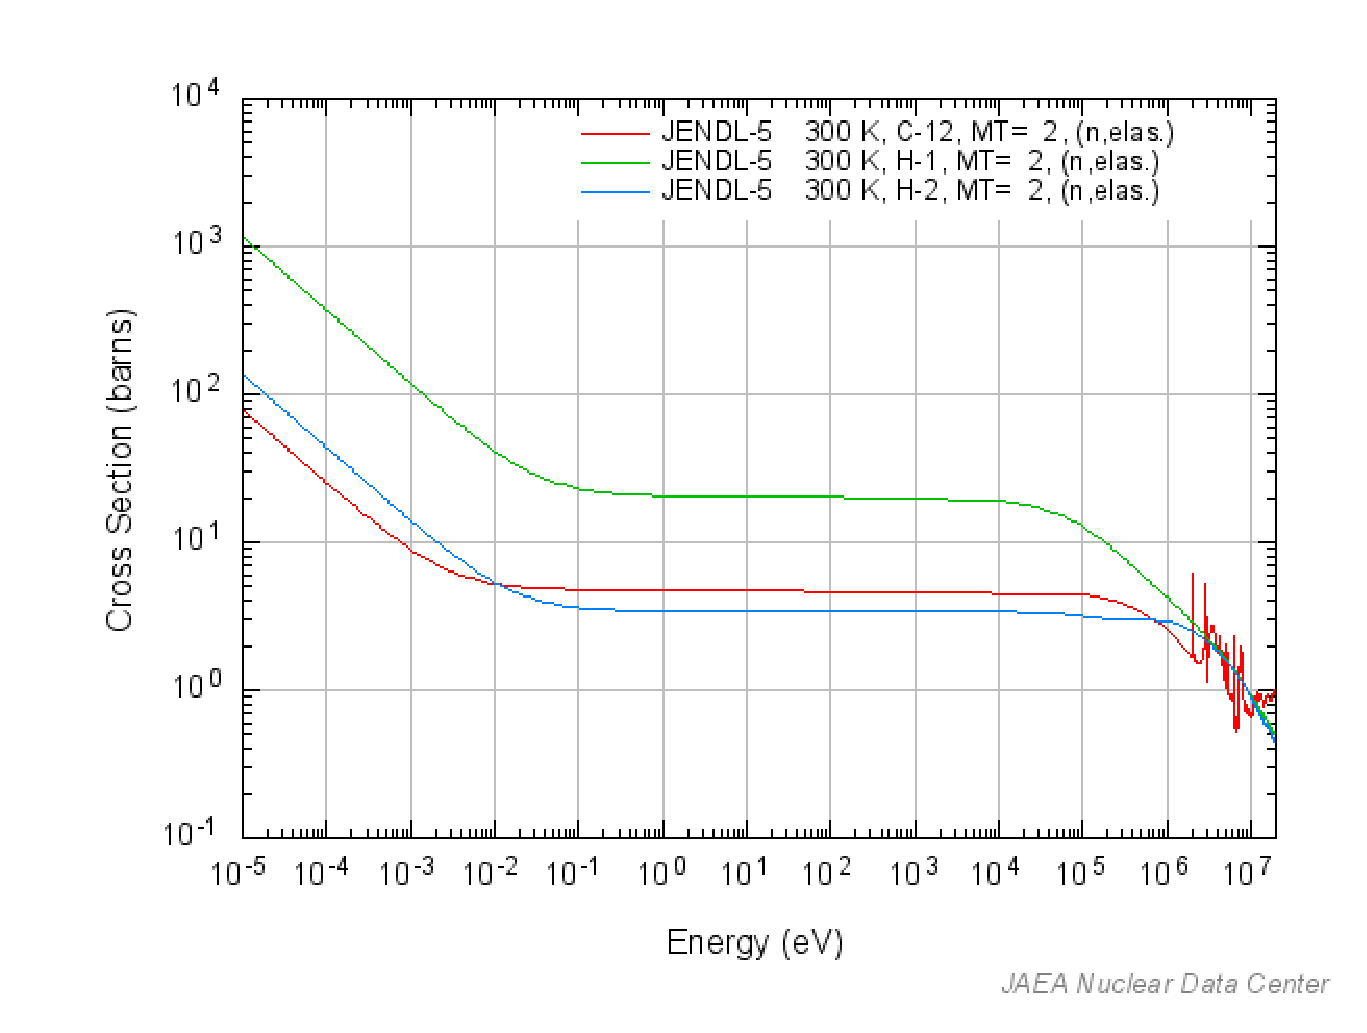
\includegraphics[width=0.8\textwidth]{figure/CrossSecElastic.eps}
  \caption{\ce{^{12}C},\ce{^{1}H},\ce{^{2}H}の弾性散乱(MT=2)の断面積}
  \label{fig:neutron_scattering}
\end{figure}

\begin{figure}[htbp]
  \centering
  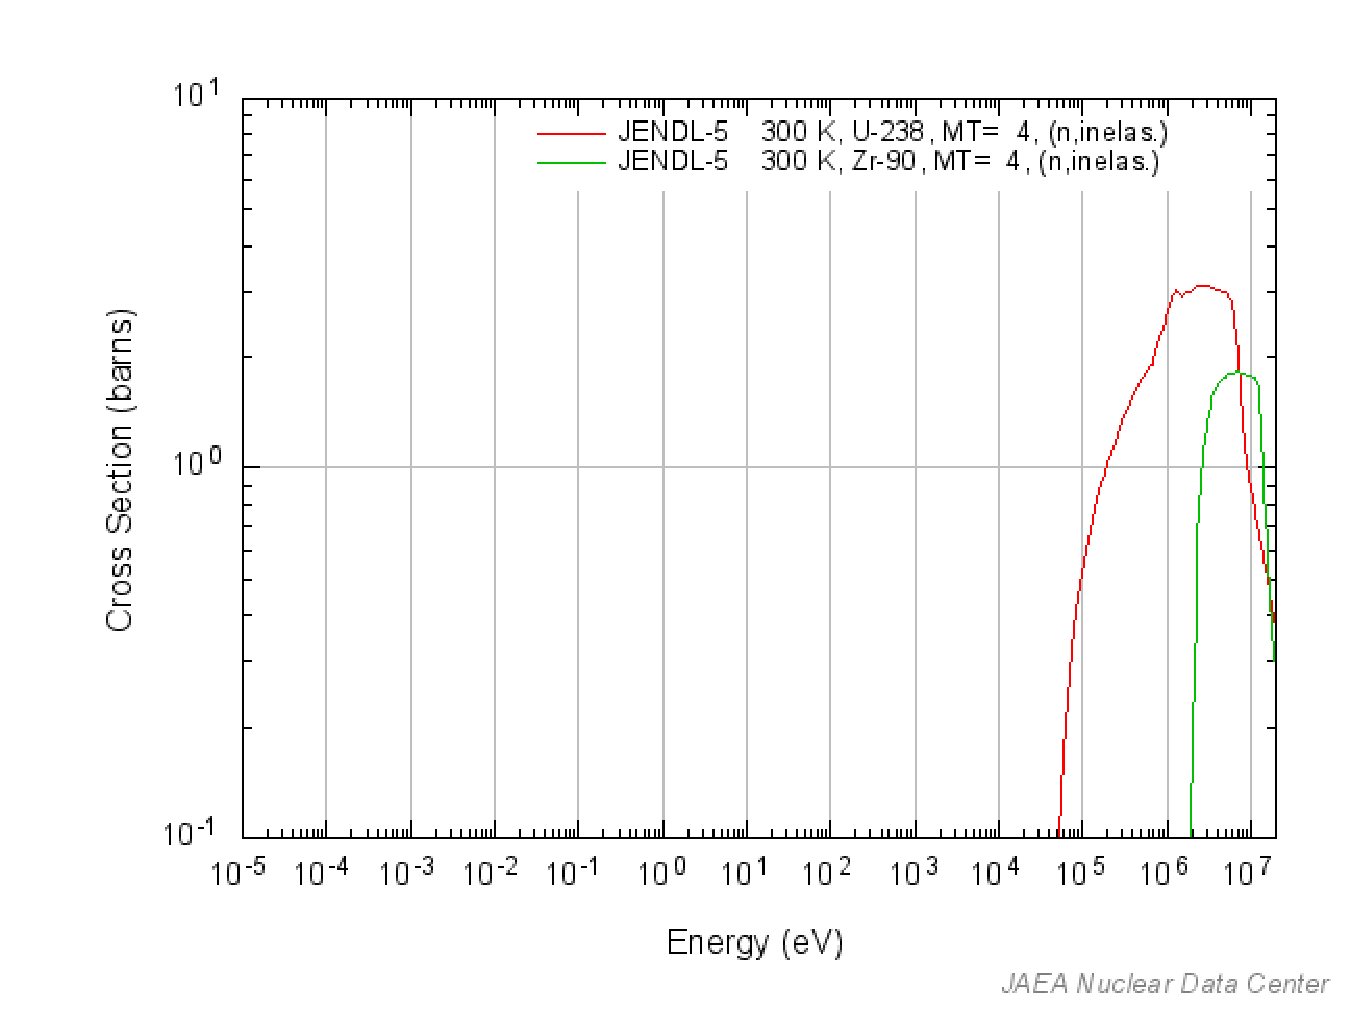
\includegraphics[width=0.8\textwidth]{figure/U238Zr90Inela.eps}
  \caption{\ce{^{238}U},\ce{^{90}Zr}の非弾性散乱(MT=4)の断面積}
  \label{fig:neutron_inelastic_scattering}
\end{figure}

\begin{figure}[htbp]
  \centering
  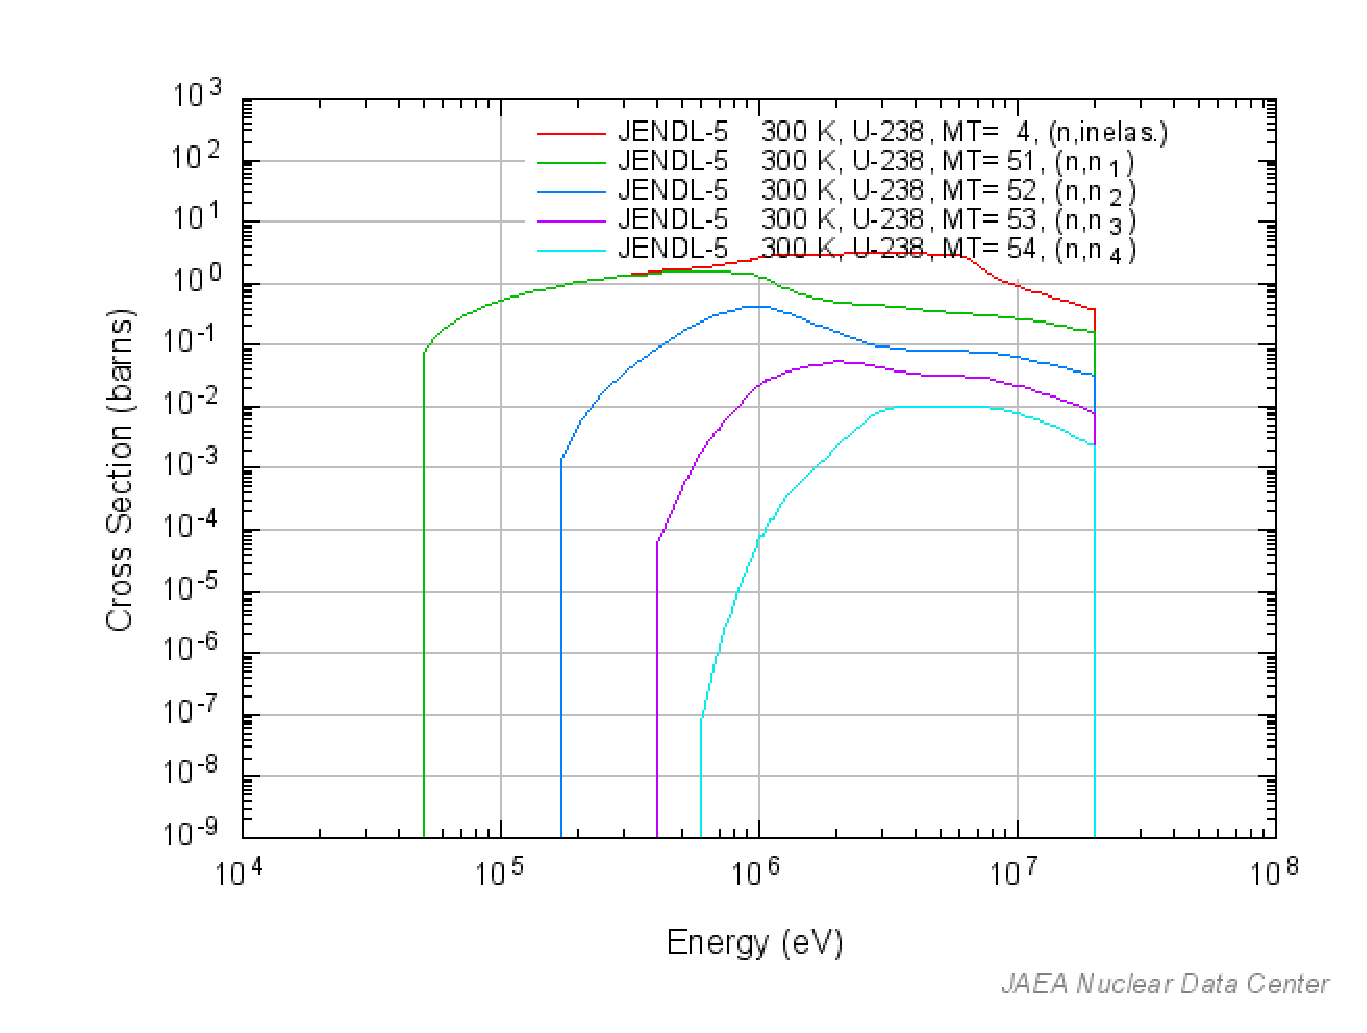
\includegraphics[width=0.8\textwidth]{figure/U238Inela_nx.eps}
  \caption{\ce{^{238}U}の非弾性散乱(MT=4,51,52,53,54)の断面積}
  \label{fig:neutron_inelastic_scattering_U238}
\end{figure}


\subsubsection{吸収反応}
原子核に中性子が取り込まれると、入射中性子のエネルギーと中性子の結合エネルギーの和の分だけ励起された複合核
が形成される。この複合核は不安定であるため、その後様々な反応を起こして安定な状態に戻ろうとする。
吸収反応この過程を経る反応の総称(散乱反応は除く)でその後の反応によってさらに多くの種類に分けられる。
これに分類されるものとしては、複合核から$\gamma$線を放出する放射捕獲反応、荷電粒子を放出する荷電粒子放出反応などがある。
原子炉において利用される核分裂反応や、入射中性子のエネルギーが高い場合に起こる2個以上の中性子が放出される反応も
この吸収反応に分類される。
Fig.~\ref{fig:neutron_absorption_Sm149}は、\ce{^{149}Sm}の(n,$\gamma$)反応、
Fig.~\ref{fig:neutron_capture_B10}は\ce{^{10}B}の(n,$\alpha$)反応、
Fig.~\ref{fig:neutron_fission}は\ce{^{235}U}の核分裂反応の断面積を示している。

それぞれの反応で共通して、低エネルギー領域では$1/v$に比例して断面積は減少している。
共鳴を持つ核種では中エネルギー領域で共鳴を起こすことも共通しているが、高エネルギー領域では捕獲断面積
は単調に減少するのに対し、核分裂断面積は階段状に増加することが分かる。
これは高エネルギーの中性子による核分裂反応では、中性子が吸収されてからすぐには割れず、1つ以上の中性子を
放出してから核分裂を起こす、マルチチャンス核分裂が存在するためである。
Fig.~\ref{fig:neutron_fission_U238}は、\ce{^{238}U}の核分裂反応において、分裂前に放出される
中性子の数ごとに分けた断面積(MT=19,20,21)と、すべての核分裂断面積の和(MT=18)を示している。

\begin{figure}[htbp]
  \centering
  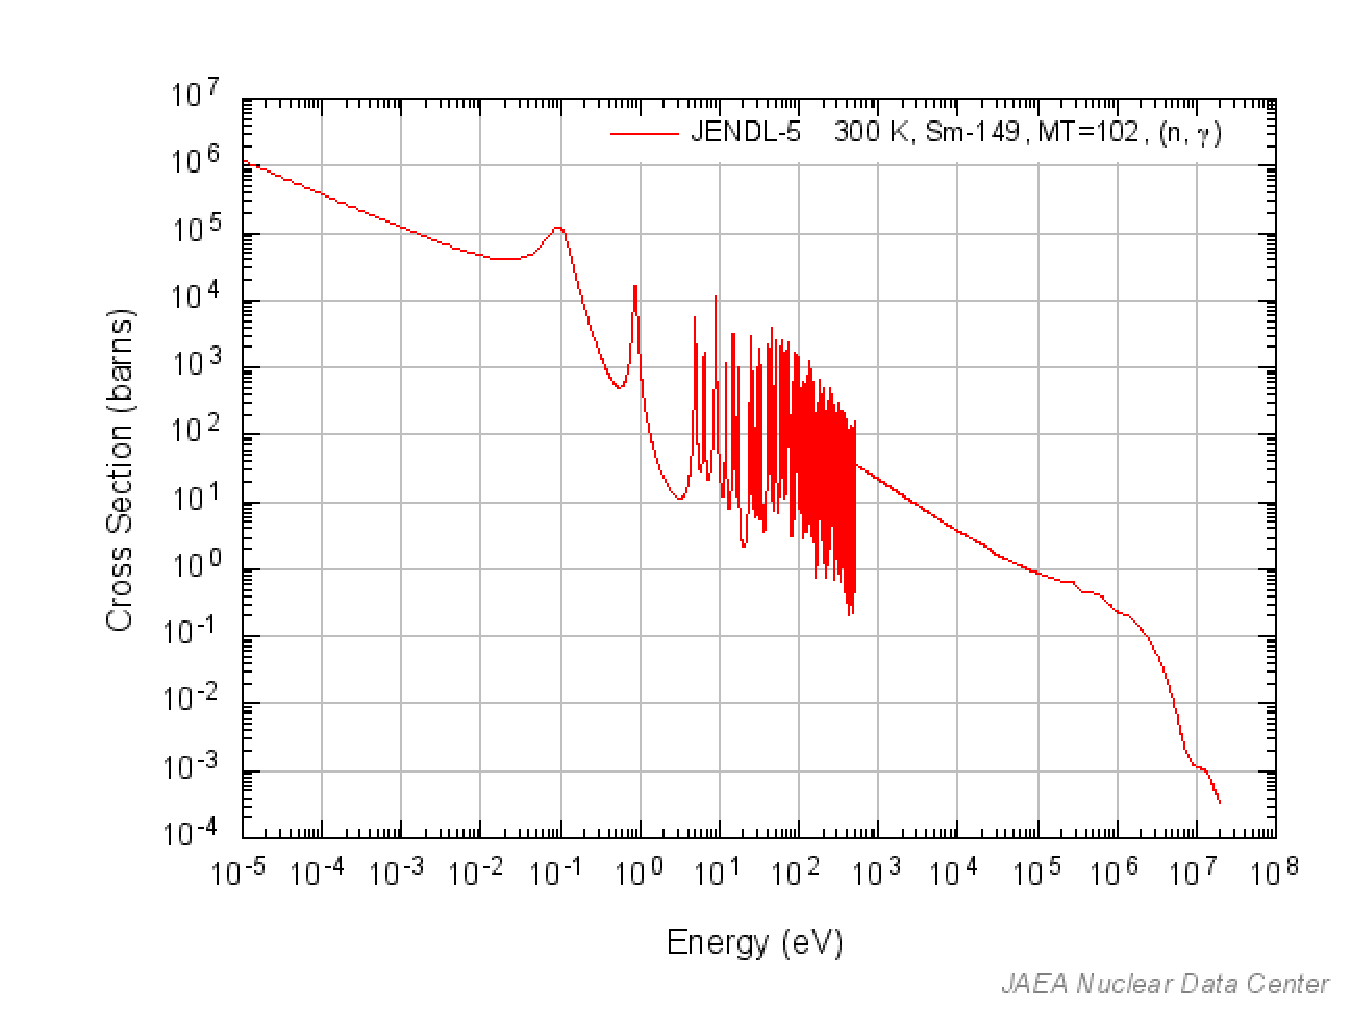
\includegraphics[width=0.8\textwidth]{figure/SmMT102.eps}
  \caption{\ce{^{149}Sm}の吸収反応(MT=102)の断面積}
  \label{fig:neutron_absorption_Sm149}
\end{figure}

\begin{figure}[htbp]
  \centering
  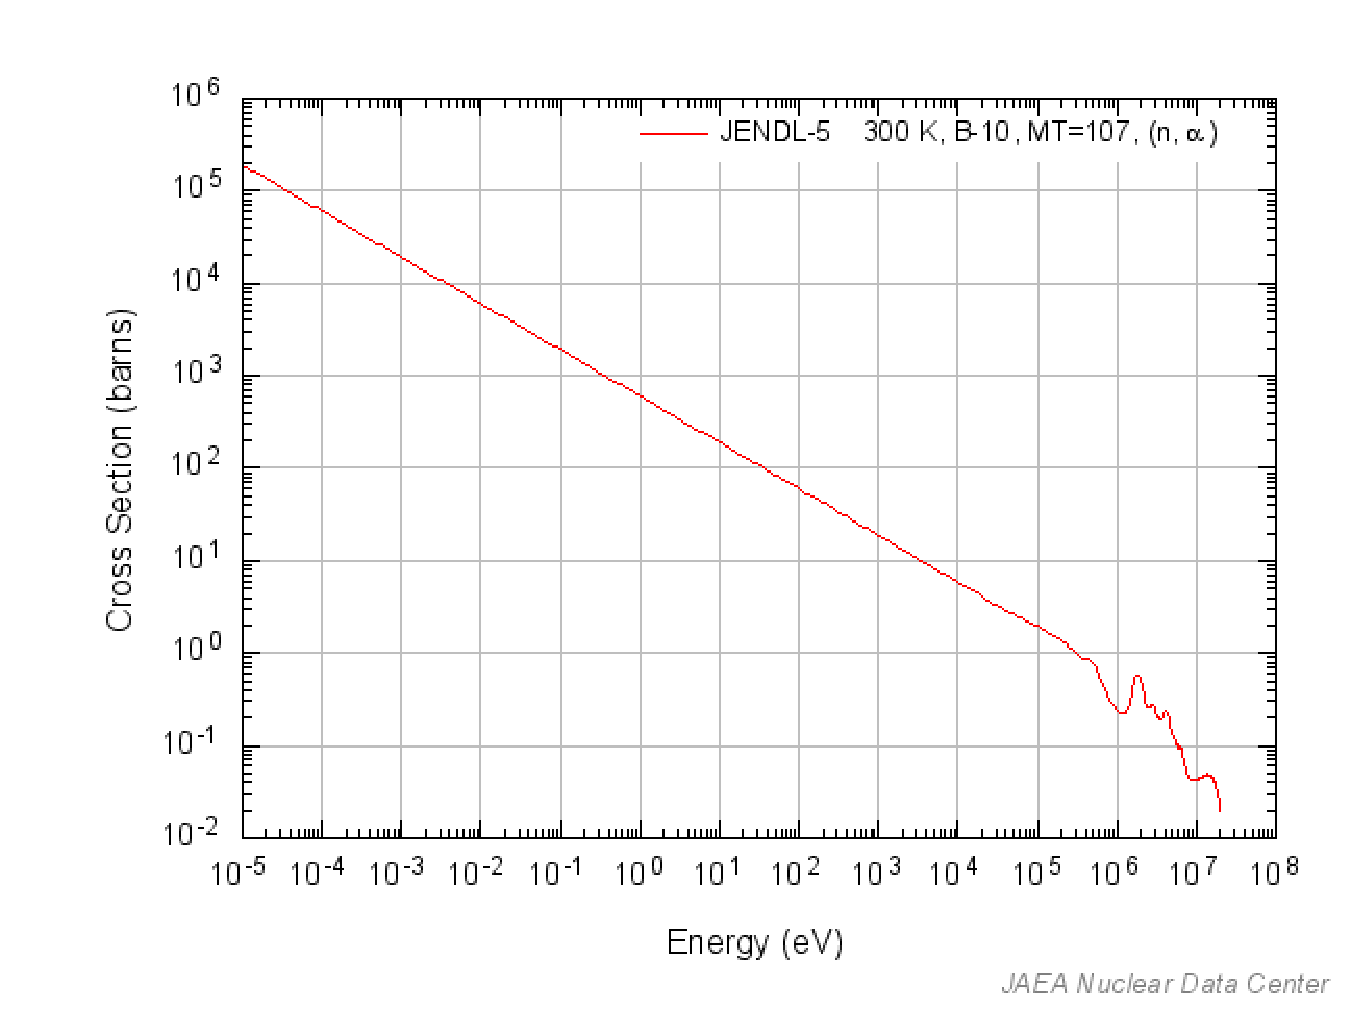
\includegraphics[width=0.8\textwidth]{figure/B10MT107.eps}
  \caption{\ce{^{10}B}の吸収反応(MT=107)の断面積}
  \label{fig:neutron_capture_B10}
\end{figure}

\begin{figure}[htbp]
  \centering
  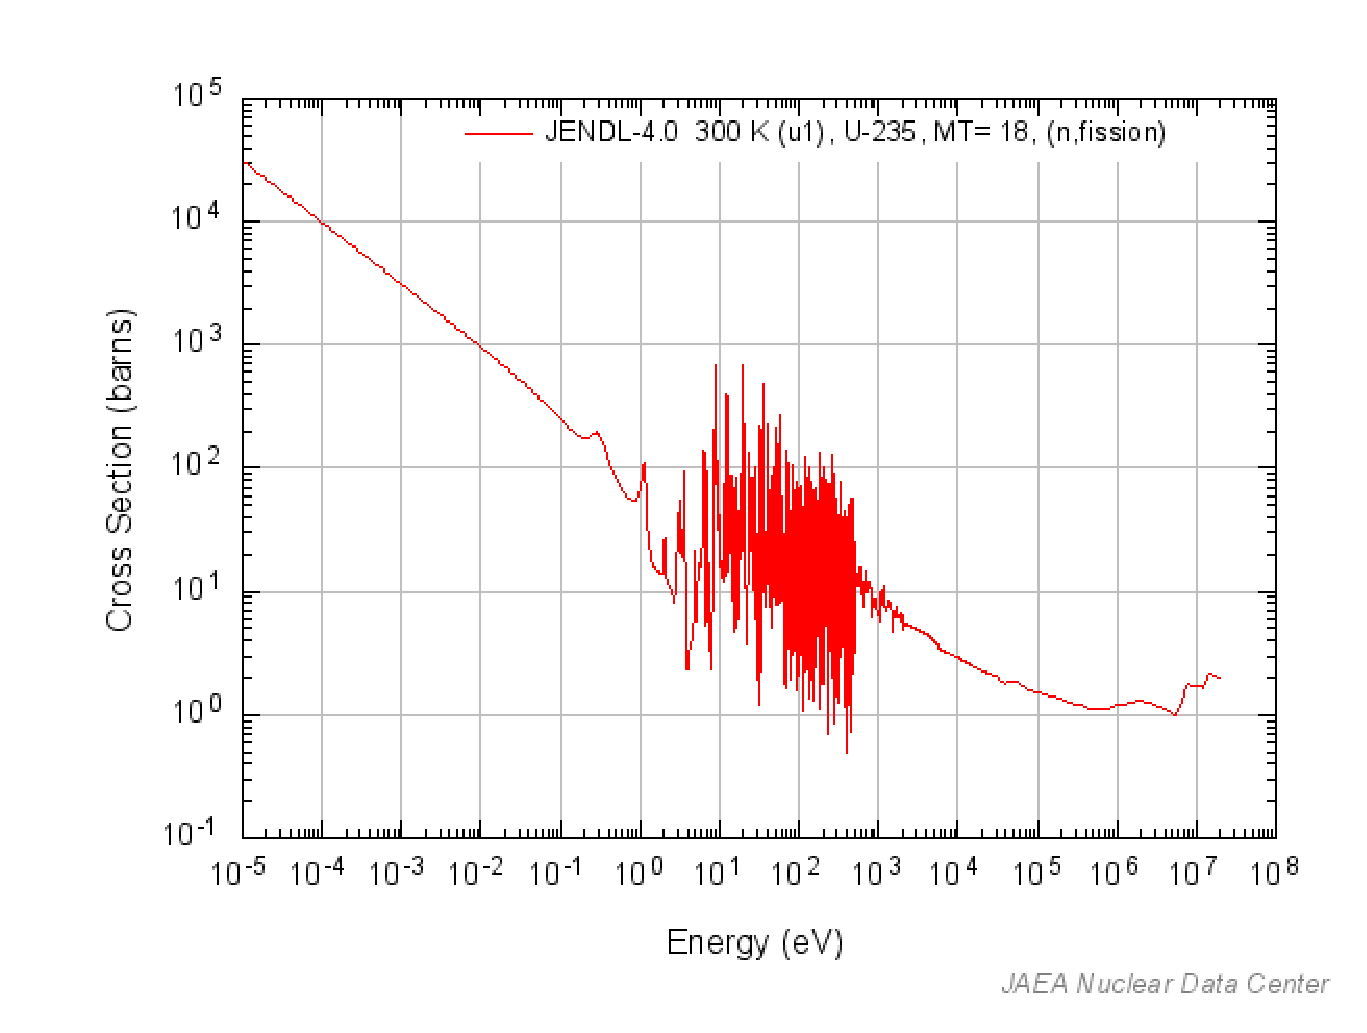
\includegraphics[width=0.8\textwidth]{figure/U235Fission.eps}
  \caption{\ce{^{235}U}の核分裂反応(MT=18)の断面積}
  \label{fig:neutron_fission}
\end{figure}

\begin{figure}[htbp]
  \centering
  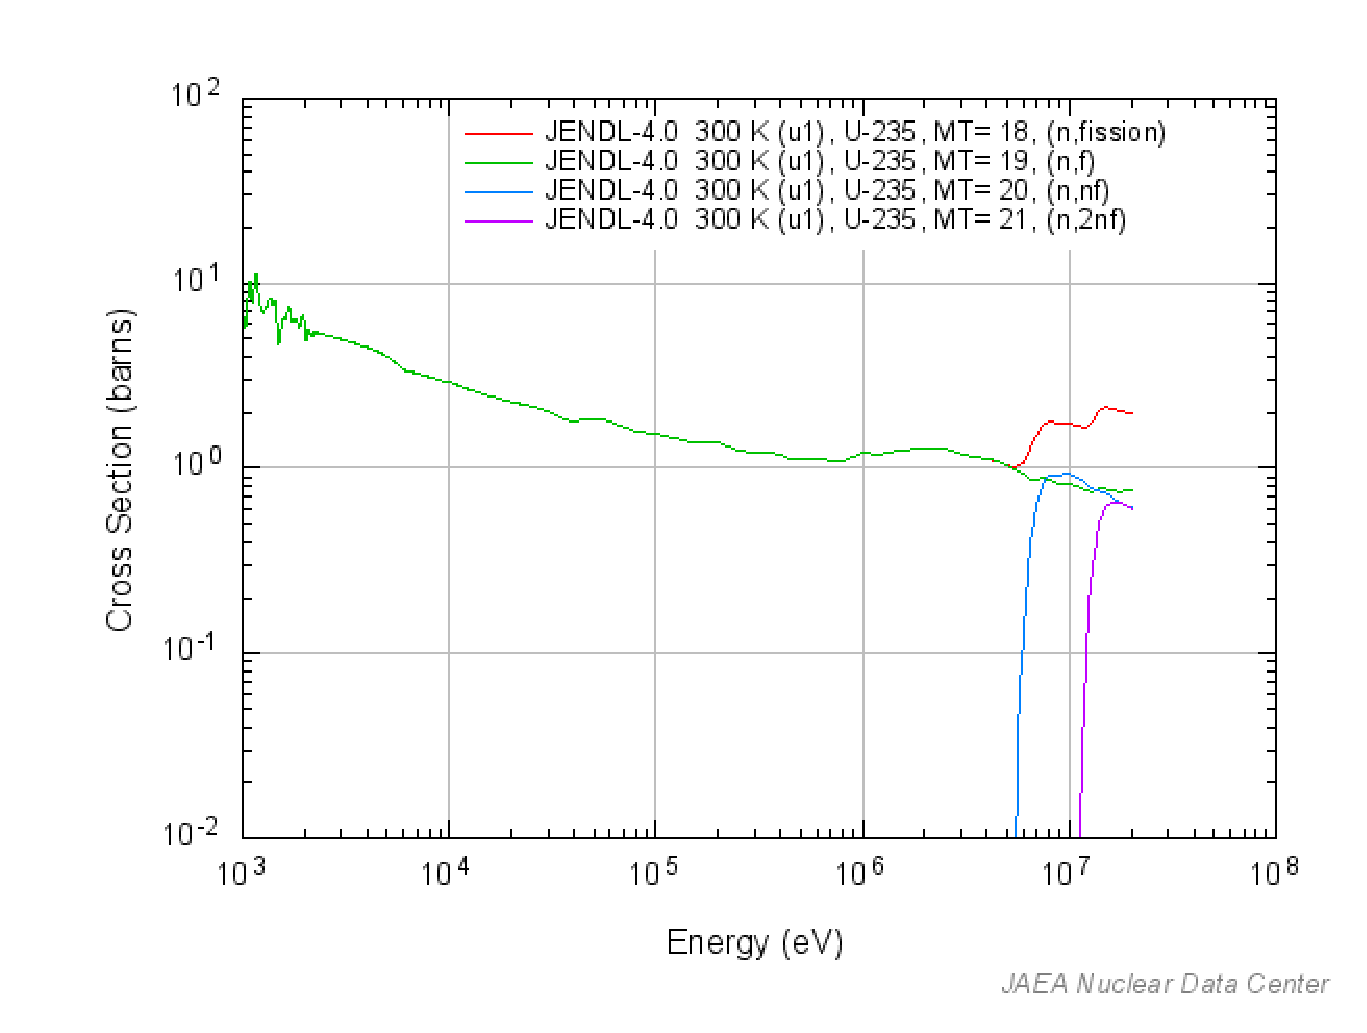
\includegraphics[width=0.8\textwidth]{figure/U235Fiss_xnf.eps}
  \caption{\ce{^{235}U}の核分裂反応(MT=18,19,20,21)の断面積}
  \label{fig:neutron_fission_U238}
\end{figure}

\clearpage

\subsection{臨界}
\ref{subsec:multipilication_factor}節で述べたように、臨界状態では中性子増倍率$k$は1で、
核分裂連鎖反応は外部から中性子を供給すること無しに、時間とともに増えも減りもせず一定の状態に維持される。
臨界を実現するための条件を調べるためにはFig.~\ref{fig:neutron_cycle}に示すような核分裂で発生した中性子の一生を考えることが適当である。

\begin{figure}[h]
  \centering
  \includegraphics[width=0.8\textwidth]{figure/neutron_cycle.eps}
  \caption{核分裂連鎖反応のサイクル}
  \label{fig:neutron_cycle}
\end{figure}

ある大きさの核分裂物質を含む体系を考える。
核分裂で発生したある世代の中性子は、体系から漏れるか、体系内にとどまるかのいずれかである。
体系にとどまる確率を$P_\text{NL}$とする。
体系にとどまった中性子は燃料に吸収されるか、燃料以外の物質に吸収されるかのいずれかである。
吸収されるとした場合に燃料に吸収される確率を$P_\text{aF}$とする。
燃料に吸収されたあと、それが捕獲反応ではなく核分裂反応を起こす確率を$P_\text{f}$とする。
核分裂を起こすと中性子を$\nu$個放出し、以下この過程を繰り返す。
\ref{eq:multi_factor}式より、増倍率$k$は次のように表される。
\begin{equation}
  k = P_\text{NL} \cdot P_\text{aF} \cdot P_\text{f} \cdot \nu
\end{equation}
以下この式をさらに定量的に考える。

\subsubsection{熱中性子利用率}
まず中性子が吸収される場合に、燃料に吸収される確率$P_\text{aF}$を考える。
燃料に吸収される確率は、燃料の中性子吸収断面積$\Sigma_\text{a}^{F}$と、
体系全体の中性子吸収断面積$\Sigma_\text{a}$の比で表される。
\begin{equation}
  P_\text{aF} = \frac{\Sigma_\text{a}^{F}}{\Sigma_\text{a}}
\end{equation}

この量を\emph{熱中性子利用率}(thermal utilization factor)と呼び$f$という記号で表す。
\begin{equation}
  f = P_\text{aF} = \frac{\Sigma_\text{a}^{F}}{\Sigma_\text{a}}
\end{equation}

\subsubsection{$\eta$(イータ)}
次に、燃料に吸収された中性子が核分裂を起こす確率$P_\text{f}$を考える。
$P_\text{f}$は燃料に吸収されたときに核分裂を起こす確率であるから、
燃料の核分裂断面積$\Sigma_\text{f}^{F}$と燃料の中性子吸収断面積$\Sigma_\text{a}^{F}$の比で表される。
\begin{equation}
  P_\text{f} = \frac{\Sigma_\text{f}^{F}}{\Sigma_\text{a}^{F}}= \frac{\sigma_\text{f}^{F}}{\sigma_\text{a}^{F}}
\end{equation}

核分裂を起こすと平均して$\nu$個の中性子が放出されるので、核燃料により中性子が再生される割合を
記号$\eta$で次のように表す。
\begin{equation}
  \eta = \nu \cdot \frac{\sigma_\text{f}^{F}}{\sigma_\text{a}^{F}} = \nu P_\text{f}
\end{equation}

この値を\emph{再生率}(reproduction factor)と呼ぶ。

\subsubsection{無限増倍率}
以上の値を用いて、増倍率$k$を書き直すと次のようになる。
\begin{equation}
  k = P_\text{NL} \cdot f \cdot \eta
\end{equation}

$P_\text{NL}$は体系の形に依存するため考えるのが難しい。そこで無限に大きい原子炉を考えて$P_\text{NL}$を1とする。
この時の増倍率を\emph{無限増倍率}(infinite multiplication factor)と呼び、記号$k_\infty$で表す。
\begin{equation}
  k_\infty = f \cdot \eta
\end{equation}

実際には$P_\text{NL}$は1より小さいため、$k_\infty > 1$でない限り原子炉が臨界になることは無い。

\subsubsection{高速中性子核分裂因子}
以上の式では、熱中性子による核分裂のみが考えられているが、
原子炉では高速中性子による核分裂も利用される。これはその世代の中性子の数をすこし増やす。
この硬化を表す量を高速中性子核分裂因子(fast fission factor)と呼び、記号$\epsilon$で表す。
\begin{equation}
  \epsilon = \frac{\text{高速および熱中性子による全核分裂中性子数}}{\text{熱中性子による核分裂中性子数}}
\end{equation}

\subsubsection{共鳴を逃れる確率}
また、中性子が発生直後の高速領域から熱領域まで減速する過程で、\ce{^{238}U}のような
共鳴を持つ核種に吸収されて失われることも考慮する必要がある。
減速過程で吸収されずに熱中性子領域まで減速される中性子の割合を\emph{共鳴を逃れる確率}(resonance escape probability)と呼び、
記号$p$で表す。

この量は燃料と減速材の割合に大きく依存するとともに、その形状、配列にも依存する。

\subsubsection{4因子公式と6因子公式}
以上の値を用いて増倍率$k$を表すと、次のようになる。
\begin{equation}
  k_\infty = \epsilon \cdot p \cdot \eta \cdot f
\end{equation}

この無限増倍率を表す式を\emph{4因子公式}と呼ぶ。
さらに中性子が体系から漏れない確率$P_\text{NL}$を、高速中性子の漏れない確率$P_\text{FNL}$
と熱中性子の漏れない確率$P_\text{TNL}$に分けると増倍率の式は次のように書き直せる。
\begin{equation}
  k = k_\infty P_\text{NL} =\epsilon \cdot p \cdot \eta \cdot f
\cdot P_\text{FNL} \cdot P_\text{TNL}
\end{equation}

この式を\emph{6因子公式}と呼び、この$k$を\emph{実効増倍率}(effective multiplication factor)と呼ぶ。

% 章ごとの参考文献欄
\printbibliography[segment=\therefsegment,heading=subbibliography]

\newpage

\section{中性子輸送}

\subsection{中性子輸送の位置づけ}
原子炉物理が原子炉内の中性子の挙動と原子核の反応を予測する学問であるとすれば、中性子輸送は
その中核をなす部分である。中性子の挙動は中性子輸送そのものであるし、原子核の反応を予測するには
中性子の分布を知ることが必須である。原子核の反応を正確に予測することができれば、核燃料の燃焼が
進んだ時の炉心の中性子の挙動を予測でき、更に先の炉心状態を予測する繰り返し作業が良い精度で
できるようになる。

ある核種$i$について炉心内での量(数密度$N_i$)の増減を予測するには、生成・消滅に関する次の方程式を解けばよい。
\begin{align}
  \frac{dN_i}{dt} &= (\text{生成率}) + (\text{変換率}) + (\text{消滅率}) \notag \\
  &= 
%  \sum_j \gamma_{ji} \sigma_{f,j} N_j \phi 
%  + \sigma_{c,i-1} N_{i-1} \phi 
%  + \sum_k \lambda_k N_k \notag \\
%  &\quad - \sigma_{a,i} N_i \phi 
%  - \lambda_i N_i \notag \\
  \begin{aligned}
    &\underbrace{\sum_j \gamma_{ji} \sigma_{f,j} N_j \phi}_{\text{核種$j$の\emph{核分裂による生成の総和}}} 
    + \underbrace{\sigma_{c,i-1} N_{i-1} \phi}_{\text{核種$i-1$の\emph{捕獲による生成}}} \\
    &+ \underbrace{\sum_k \lambda_k N_k}_{\text{核種$k$の\emph{崩壊による生成の総和}}} 
    - \underbrace{\sigma_{a,i} N_i \phi}_{\text{核種$i$の\emph{吸収による変換}}} 
    - \underbrace{\lambda_i N_i}_{\text{核種$i$の\emph{崩壊による消滅}}}
  \end{aligned}
  \label{BurnupEq}
\end{align}

この式~\eqref{BurnupEq}は\emph{燃焼方程式}と呼ばれる連立の一階常微分方程式である。
全ての核種の数密度をベクトルとして見ると、この式は
\begin{align}
  \frac{d\mathbf{N}}{dt} = \mathbf{A} \mathbf{N}  \label{BurnupEq2}
\end{align}
と表記できる。この$\mathbf{A}$は「燃焼マトリックス」と呼ばれる行列である。
燃焼マトリックス内の各反応率が全て一定であれば、
式~\eqref{BurnupEq2}の解析解は
\begin{align}
  \mathbf{N}(t) = \mathbf{N}(0) \exp{ (\mathbf{A} t) } \label{BurnupEqAnlSol}
\end{align}
である。実際には、数密度は位置によって異なるはずなので、ここで求まる$\mathbf{N}(t)$は「\emph{ある位置}、
ある時刻の核種数密度$\mathbf{N}(\mathbf{r},t)$」とすべきであるし、燃焼マトリックスについても
中に出てくる$\phi$が、「\emph{ある位置、ある時刻}の中性子束$\phi(\mathbf{r},t)$」であるため、
反応率は位置や時間によって変化する。したがって、実際の原子炉の解析では時間的・空間的な
\emph{離散化}を施すことになる。
\begin{figure}[htbp]
  \begin{center}
  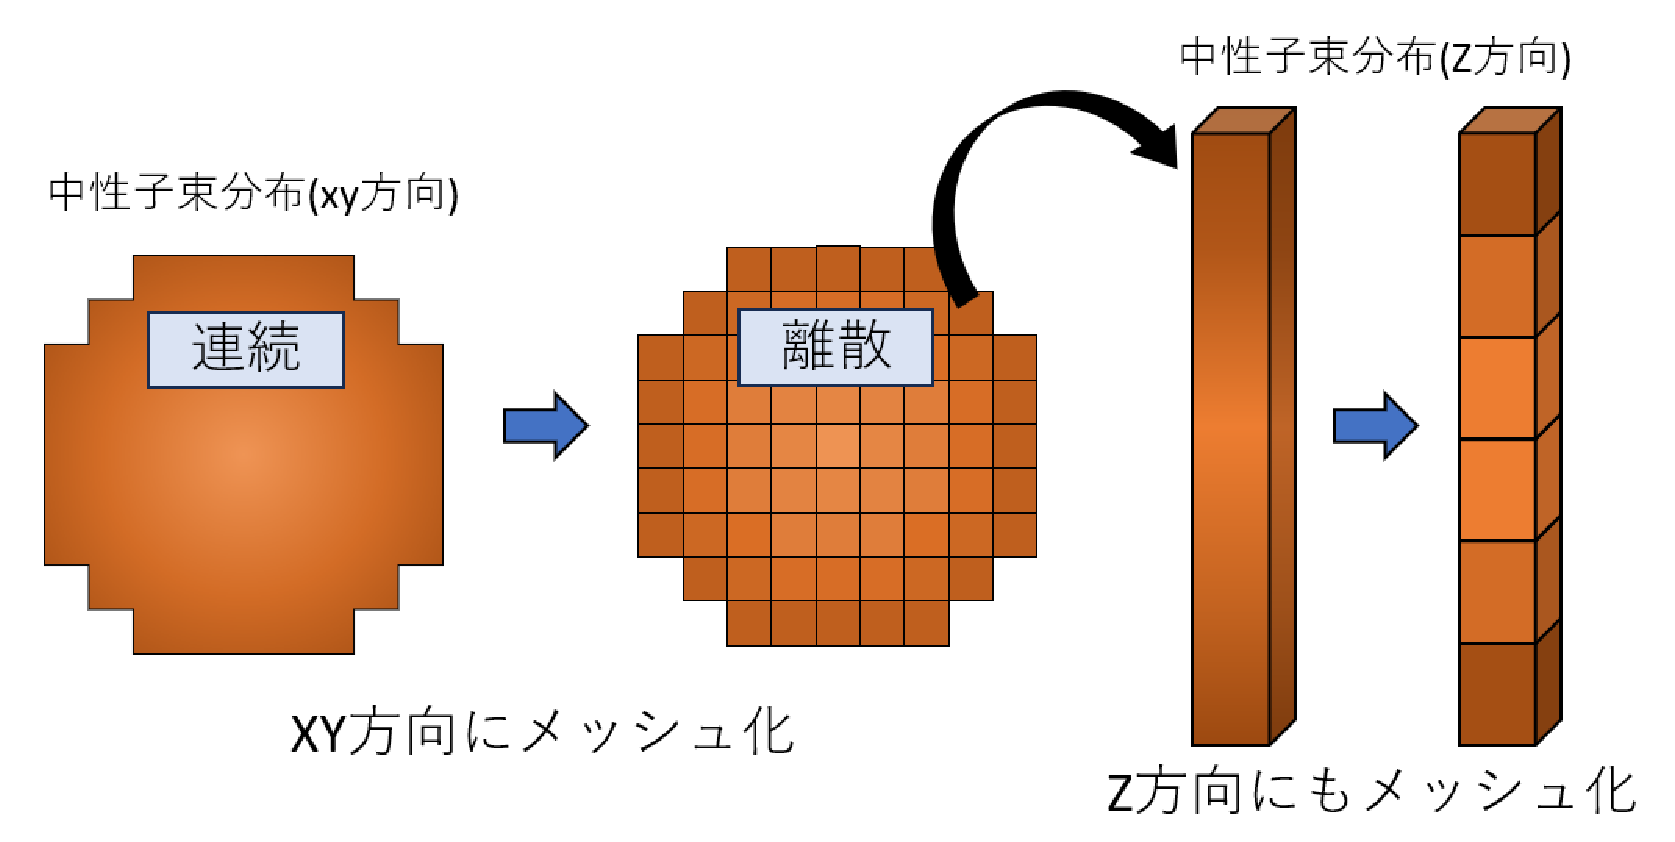
\includegraphics[width=100mm]{figure/discretization.eps}
  \caption{炉心の中性子束分布をメッシュ化して空間的に離散化する}\label{discretization}
  \end{center}
\end{figure}
\begin{figure}[htbp]
  \begin{center}
  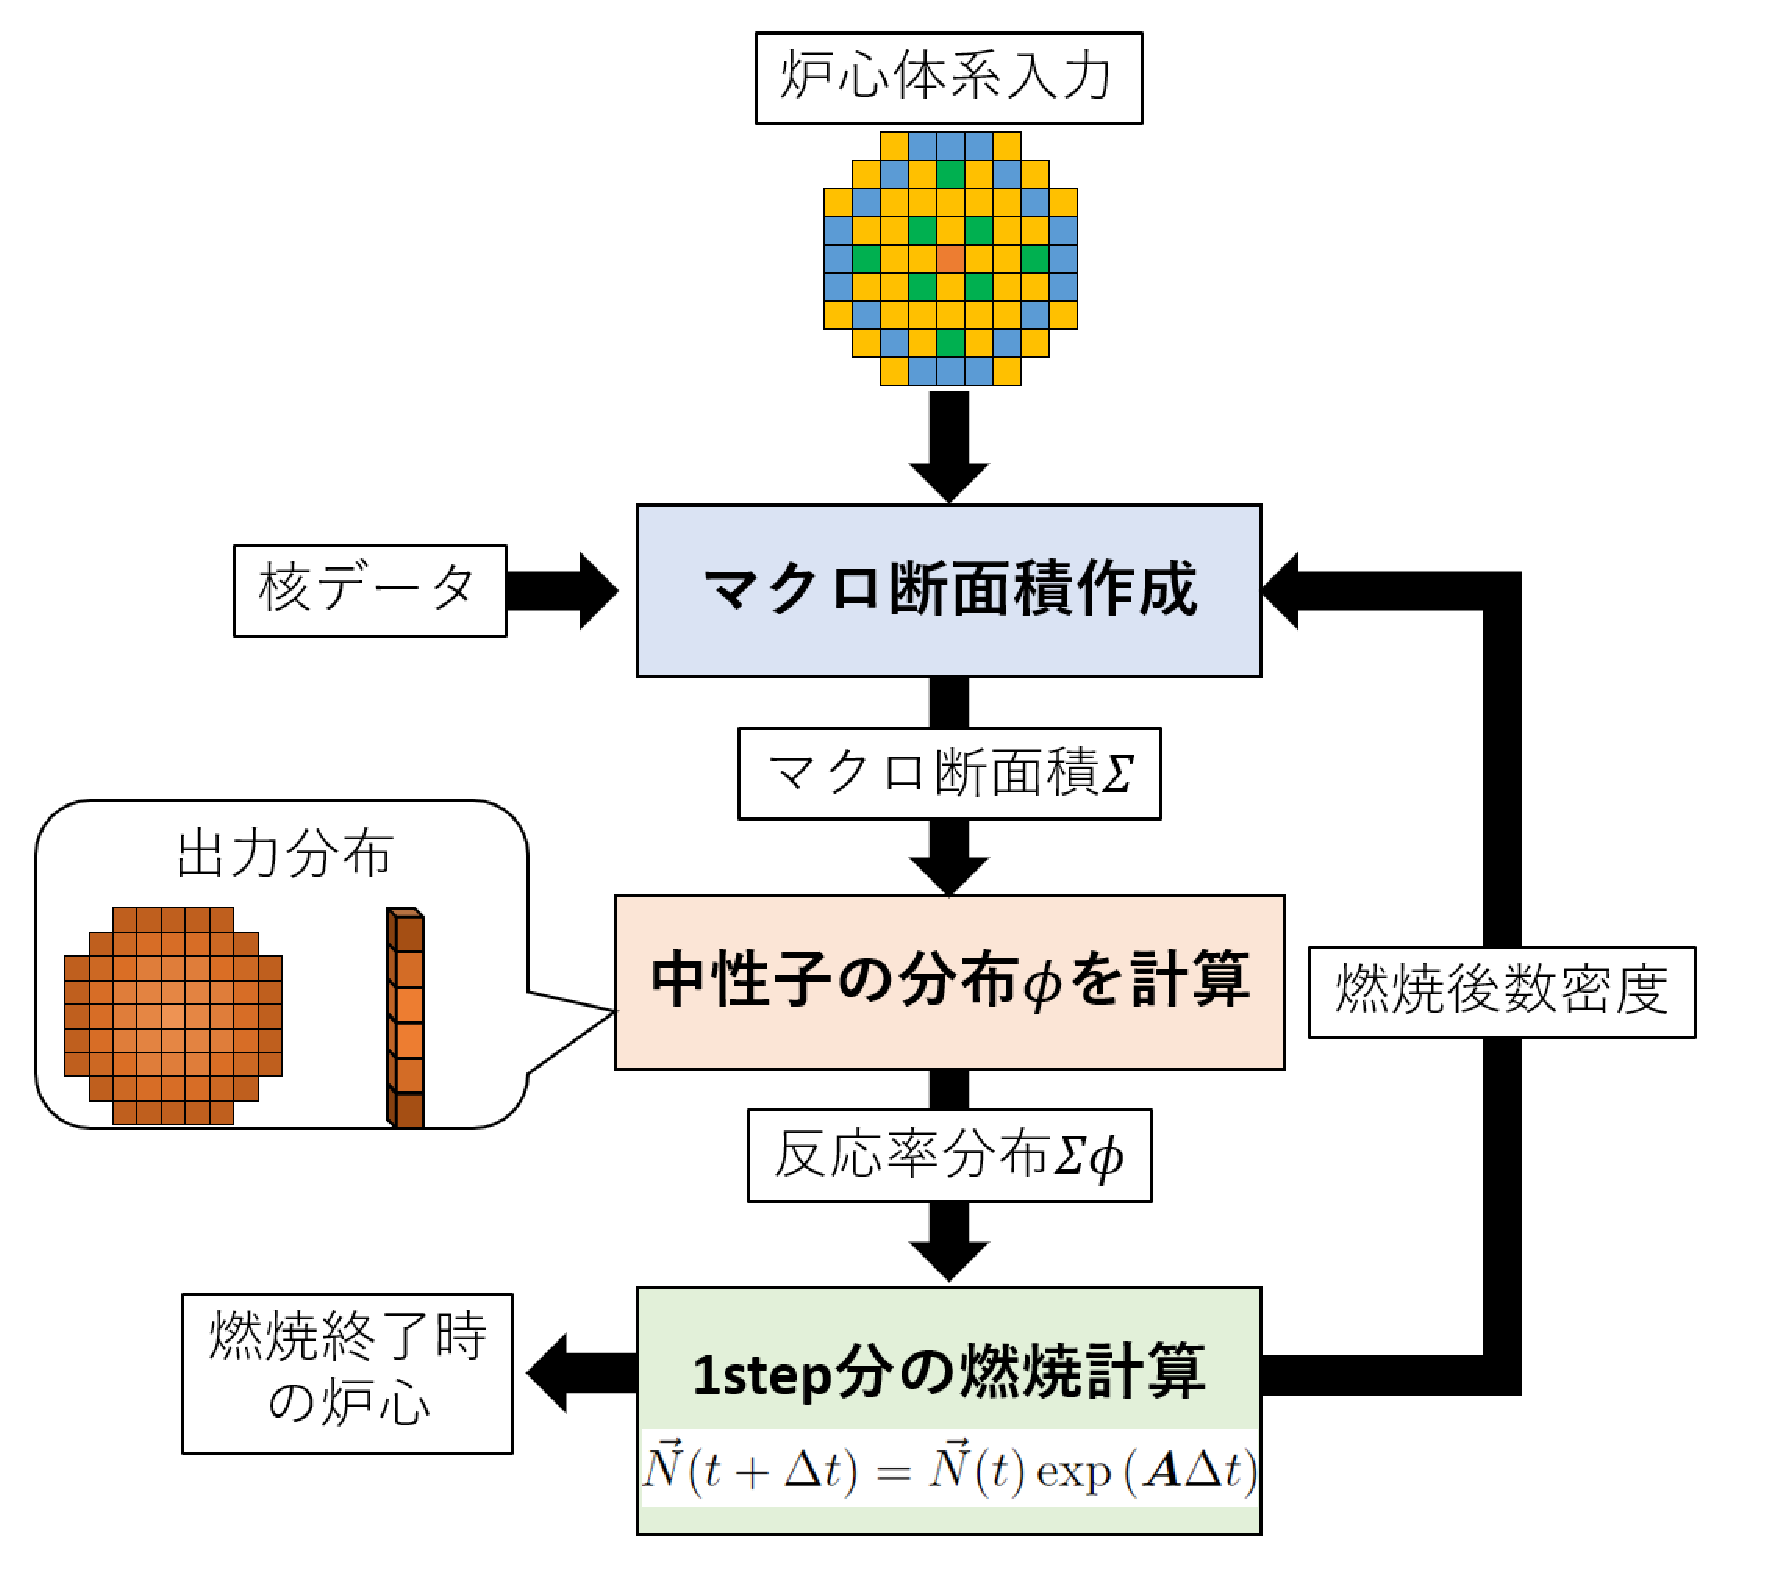
\includegraphics[width=100mm]{figure/time-discretization.eps}
  \caption{燃焼サイクルの時間的離散化}\label{time-discretization}
  \end{center}
\end{figure}
\begin{comment}
\begin{align}
  \Delta\mathbf{N} = \mathbf{A} \mathbf{N} \Delta t   \label{BurnupEqDis}
\end{align}
\begin{align}
  \mathbf{N}(t + \Delta t) = \mathbf{N}(t) \exp{( \mathbf{A} \Delta t )} \label{BurnupEqDisSol}
\end{align}
\end{comment}
Fig.~\ref{discretization}、Fig.~\ref{time-discretization}はPWRや高速炉の
炉心計算の離散化例である。XYZ方向に区切られたメッシュ内で、中性子束や燃料組成を
均一とする空間的離散化を適用し、計算条件として与えている。
時間については、\emph{燃焼サイクルを複数のステップに区切り、その期間内の反応率
が一定であるとみなし}離散化している。各燃焼ステップごとに中性子束分布が
変化するため、ステップ毎に中性子輸送計算を実施し、これを基にステップ後の燃料組成を
求めるという作業を繰り返すことになる。炉心設計では多数の炉心を計算するため、
計算時間の短縮が大きな課題となっている。計算の高速化にはメッシュや燃焼ステップを
大きくし、扱うデータ数と計算反復数を減らす必要があるが、計算で生じた誤差が後の
燃焼ステップに影響し蓄積していく性質があるため、高精度の予測には細かい離散化が
必要になるトレードオフが存在する。そこで、中性子輸送計算を高速かつ高精度に計算する
手法がこれまでに研究されてきた。

もっとも、細かい計算手法について取り扱う時間はないので、
今回のゼミでは中性子束分布の計算に必要な中性子輸送方程式と、
最も基本的な近似である中性子拡散方程式を取り扱うこととする。












\subsection{中性子束と中性子流}
原子炉物理の中で頻出する単語に「\emph{中性子束}」があり、このパラメータは
一般に$\phi$で示す。これとよく似た単語に「\emph{中性子流}」があり、紛らわしい。
ここではまずこの基本的な2つのパラメータについて説明する。

\subsubsection{角度中性子密度}
\newcommand{\SpcAng}{\mathbf{\hat{\Omega}}} % 飛行方向の単位ベクトル
\newcommand{\rEOt}{\mathbf{r}, E, \SpcAng, t} % 文字の()内変数
ある座標$\mathbf{r}$で、あるエネルギー$E$を持ちある方向$\SpcAng$に飛行する中性子の、
ある時刻$t$においての密度を「\emph{角度中性子密度}(angular neutron density)」
$n(\rEOt)$と呼び、次のように定義される。なお$\SpcAng$は飛行方向の単位ベクトルである。
\begin{align}
  n(\rEOt) dVdEd\SpcAng &= 
  \left(
  \begin{aligned}
    &\quad\text{時刻$t$に、} \\
    &\quad\text{位置$\mathbf{r}$まわりの体積$dV$内に存在し、}\\
    &\quad\text{エネルギーが$E$まわりの幅$dE$内にあり、} \\
    &\quad\text{方向$\SpcAng$まわりの$d\SpcAng$に向かって飛行する}\\
    &\quad\text{中性子数の期待値}
  \end{aligned}
  \right)
  \label{AngDens}
\end{align}

\subsubsection{角度中性子束と角度中性子流}
角度中性子密度を用いて、\emph{角度中性子束}(angular neutron flux)
\footnote{平川先生の黄色の教科書では$\Phi$としているが太字っぽくて
ベクトルに見えてしまうため、代わりに使われることがある$\psi$で表記する}と
\emph{角度中性子流}(angular neutron current)を定義できる。
\begin{align}
  \text{角度中性子束} &= \psi(\rEOt) = v(E) n(\rEOt) \label{AngFlux}\\
  \text{角度中性子流} &= \mathbf{j}(\rEOt) = v(E) n(\rEOt) \SpcAng = \psi(\rEOt) \SpcAng \label{AngCrnt}
\end{align}
角度中性子束と角度中性子流はよく似ているが、\emph{束がスカラー量}で\emph{流がベクトル量}であるという
根本的な違いがある。

\vskip\baselineskip
\begin{shadebox}
  \vskip.5\baselineskip
  \toi 角度中性子流について
  \begin{align}
    \mathbf{j}(\rEOt) d\mathbf{A} dE d\SpcAng \notag
  \end{align}
  という積はどのような物理的意味を持つだろうか。\\
  なお、$d\mathbf{A}$は「位置$\mathbf{r}$にある微小な面」として定義される面要素であり、
  この面に垂直な単位ベクトル$\mathbf{e_s}$を用いて
  $d\mathbf{A} = \mathbf{e_s} \cdot dA$で定義される。\\
\end{shadebox}
\begin{comment}
  時刻$t$に
  エネルギーが$E$まわりの幅$dE$内にあり、
  方向$\SpcAng$まわりの$d\SpcAng$に向かって飛行する中性子が
  単位時間に
  面$d\mathbf{A}$を通過する期待値
\end{comment}
\vskip8\baselineskip
%\newpage

\subsubsection{中性子密度、中性子束と中性子流}
\newcommand{\rEt}{\mathbf{r}, E, t} % 文字の()内変数
角度中性子密度、角度中性子束と角度中性子流をそれぞれ飛行方向で積分したのが
\emph{中性子密度}(neutron density)、\emph{中性子束}(neutron flux)と
\emph{中性子流}(neutron current)である。

\begin{align}
  \text{中性子密度} &= n(\rEt)
   = \int_{4 \pi} n(\rEOt) \ d\SpcAng \label{ndens-E}\\
  \text{中性子束} &= \phi(\rEt)
   = \int_{4 \pi} \psi(\rEOt) \ d\SpcAng \label{flux-E}\\
  \text{中性子流} &= \mathbf{J}(\rEt)
   = \int_{4 \pi} \mathbf{j}(\rEOt) \ d\SpcAng \label{crnt-E}
\end{align}

エネルギーについても積分すれば、エネルギーに依存しない各物理量を定義できる。
\newcommand{\rOt}{\mathbf{r}, \SpcAng, t} % 文字の()内変数
\newcommand{\rt}{\mathbf{r}, t} % 文字の()内変数
\newcommand{\nhat}{\mathbf{\hat{n}}} % 単位法線ベクトル
\begin{align}
  \text{中性子密度} &= n(\rt)
   = \int_{0}^{\infty} n(\rEt) \ dE \label{ndens}\\
  \text{中性子束} &= \phi(\rt)
   = \int_{0}^{\infty} \phi(\rEt) \ dE \label{flux}\\
  \text{中性子流} &= \mathbf{J}(\rt)
   = \int_{0}^{\infty} \mathbf{J}(\rEt) \ dE \label{crnt}
\end{align}

\vskip\baselineskip
\begin{shadebox}
  \vskip.5\baselineskip
  \toi 中性子束と中性子流は何が違うのだろうか。なぜ2つの似た概念を別個
  用意する必要があるのだろうか。\\
  ヒント:任意の単位ベクトル$\nhat$と中性子流の内積
  $\mathbf{n} \cdot \mathbf{J}(\rEt)$の意味は?\\
\end{shadebox}
\begin{comment}
  ある位置$\mathbf{r}$の点の中性子束、中性子流
  (エネルギーに依存しない)について考える
  中性子束は単位時間、単位面積あたりにその点を通過する中性子の総数
  中性子流は単位時間、単位面積あたりにその点を通過する正味の中性子数
  束は交通量調査で、流は正味の中性子の流れの方向と大きさを示す
  束は点から伸びる中性子の動きのベクトルの長さを足し合わせたスカラー
  流は点から伸びる中性子の動きのベクトルを全て足したベクトル
  一般的な物理学で出てくる束(磁束など)は中性子流と同様の概念で
  中性子束は原子炉物理に独特の概念である
  これは核反応は中性子の運動の方向に関係なく核反応するから
  束は核反応の量を見るための量
  流は中性子の動きを見るための量
\end{comment}
\vskip8\baselineskip
%\newpage

\subsection{中性子輸送方程式}
ここからは、定義した中性子束・中性子流から厳密に正しい中性子の輸送に関する
方程式、「\emph{中性子輸送方程式}」を導出する。

\subsubsection{中性子輸送方程式の設計図}
まず、厳密に正しい中性子輸送を記述するには何が必要かを考える、
すなわち、方程式の設計図を作成していくこととする。
出発点として、中性子輸送方程式を
\begin{itemize}[label={}]
  \item ある時刻$t$に
  \item 位置$\mathbf{r}$まわりの体積$dV$内に存在し、
  \item エネルギーが$E$まわりの幅$dE$内にあり、
  \item 方向$\SpcAng$まわりの$d\SpcAng$に向かって飛行する
  \item 中性子数の期待値
\end{itemize}
すなわち角度中性子密度$n(\rEOt)$の時間変化に着目した方程式と捉えよう。
角度中性子密度の時間変化に影響を与えるものとして、次の項目がある。
\begin{align}
  \frac{\partial n(\rEOt)}{\partial t} &= \text{角度中性子密度の時間変化} \notag \\
   &= \text{生成率} - \text{消滅率} \notag \\
   &= \text{(空間的な流入以外の)生成率} - (\text{漏洩率} + \text{吸収率} + \text{散乱で失われる率})
\end{align}

\subsubsection{生成率}
角度中性子密度を増加させる要因としては次のものが考えられる。
\vskip.5\baselineskip
\subparagraph{中性子源による生成}
位置$\mathbf{r}$まわりの体積$dV$内に中性子源がある場合、
中性子数は増加する。線源によって$n(\rEOt)$にカウントされる
中性子を放出する数を$s(\rEOt)$とする。
これを\emph{中性子線源項}と呼ぶ。
\begin{itembox}[l]{中性子線源項}
  \begin{equation}
    \text{中性子源による生成率} = s(\rEOt) \label{source}
  \end{equation}
\end{itembox}

\newpage
\subparagraph{散乱による生成}
\newcommand{\EOtoEO}{E' \rightarrow E, \SpcAng' \rightarrow \SpcAng}
\begin{itemize}[label={}]
  \item ある時刻$t$に
  \item 位置$\mathbf{r}$まわりの体積$dV$内に存在し、
  \item 他のエネルギー$E'$周りの幅$dE'$内で
  \item 方向$\SpcAng'$まわりの$d\SpcAng'$の方向に飛行する中性子
\end{itemize}
が、散乱によって$n(\rEOt)$にカウントされる中性子になる場合も生成として捉える。
$E'$からの散乱による生成率は
\begin{align}
  \text{$E'$、$\SpcAng'$からの散乱による生成率}
   = \Sigma_s (\mathbf{r}, \EOtoEO) v(E') n(\mathbf{r}, E', \SpcAng', t)
\end{align}
エネルギーと立体角について積分すれば、散乱による生成率を表現できる。
これを\emph{散乱流入項}と呼ぶ。
\begin{itembox}[l]{散乱流入項}
  \begin{equation}
    \text{散乱による生成率}
     = \int_{4 \pi} \int_{0}^{\infty} \Sigma_s (\mathbf{r}, \EOtoEO) v(E') n(\mathbf{r}, E', \SpcAng', t) \ dE' d\SpcAng' \label{inscattering}
  \end{equation}
\end{itembox}
$\Sigma_s (\mathbf{r}, \EOtoEO)$はエネルギー依存、立体角依存の
散乱断面積であり、2重微分断面積と呼ぶ。

\subsubsection{漏洩率}
漏洩率では\emph{空間的な流入・流出}を同時に取り扱う。
領域$V$を設定し、その表面$S$の微小面積$\Delta S$を考え、その面に対する外向きの
単位法線ベクトル$\nhat$とおく。まず、$\Delta S$を
単位時間あたりに通過する$\SpcAng$方向の速さ$v$の中性子数について数式で表現する。
これは、微小面積$\Delta S$を長さ$v$だけ$\SpcAng$方向に動かした際にできる
微小体積$\Delta V$内に存在する中性子数に等しくなるはずである。よって、
正味の流量は以下で表せる。
\begin{align}
  \Delta V = v \nhat \cdot \SpcAng \Delta S \ \text{なので、}\notag \\
  n(\rEOt) v(E) \nhat \cdot \SpcAng \Delta S
\end{align}
領域$V$全体で考えるなら表面$S$で積分すればよく、
\begin{align}
  \text{領域$V$からの漏洩率} &= \int_{S} \nhat \cdot \SpcAng v(E) n(\rEOt) \ dS \notag \\
  &= \int_{S} \nhat \cdot \SpcAng \psi(\rEOt) \ dS \quad \text{ガウスの発散定理から}\\
  &= \int_{V} \mathrm{div} \ \SpcAng \psi(\rEOt) \ dV \label{V-lossterm} 
\end{align}
 $\nabla = \left( \frac{\partial}{\partial x},
 \frac{\partial}{\partial y}, \frac{\partial}{\partial z}\right)$
を用いれば、
\begin{align}
  \int_{V} \mathrm{div} \ \SpcAng \psi(\rEOt) \ dV &= \int_{V} \nabla \SpcAng \psi(\rEOt) \ dV \notag\\
  \text{$\SpcAng$が空間$\mathbf{r}=(x,y,z)$に依存しないので} \quad &= \int_{V} \SpcAng \cdot \nabla \psi(\rEOt) \ dV
\end{align}
式~\eqref{V-lossterm}を体積$V$で割り、$V \rightarrow 0$と
すると、単位体積あたりの漏洩率となる
\footnote{$\psi$がスカラー量なので$\nabla \psi$はベクトルを与える}。
\begin{itembox}[l]{漏洩率}
  \begin{equation}
    \text{漏洩率}
     = \SpcAng \cdot \nabla \psi(\rEOt) \label{lossterm-flux}
  \end{equation}
  あるいは、角度中性子流を使って
  \begin{equation}
    \nabla \cdot \mathbf{j}(\rEOt)  \label{lossterm-crnt}
  \end{equation}
\end{itembox}

\subsubsection{吸収率}
吸収される量は巨視的吸収反応断面積を$\Sigma_a$とおいて次で表される。
\begin{itembox}[l]{吸収率}
  \begin{equation}
    \text{吸収率}
     = \Sigma_a v(E) n(\rEOt) \label{absorptionterm}
  \end{equation}
\end{itembox}

\subsubsection{散乱で失われる率}
散乱で失われる量は巨視的散乱断面積を$\Sigma_s$とおいて次で表される。
\begin{itembox}[l]{散乱で失われる率}
  \begin{equation}
    \text{散乱で失われる率}
     = \Sigma_s v(E) n(\rEOt) \label{scatteringterm}
  \end{equation}
\end{itembox}

\subsubsection{微積分型中性子輸送方程式}
ここまでに表現した項を組み合わせて「微積分型」の中性子輸送方程式を
組み立てる。

\begin{align}
  \frac{\partial n(\rEOt)}{\partial t}
   &= s(\rEOt) \notag \\
   &+ \int_{4 \pi} \int_{0}^{\infty} \Sigma_s (\mathbf{r}, \EOtoEO) v(E') n(\mathbf{r}, E', \SpcAng', t) \ dE' d\SpcAng' \notag \\
   &- \left(
  \begin{aligned}
   &\quad \SpcAng \cdot \nabla \psi(\rEOt) \\
   &+ \Sigma_a v(E) n(\rEOt) \\
   &+ \Sigma_s v(E) n(\rEOt)
  \end{aligned}
   \right) \label{transport-pre}
\end{align}

式~\eqref{transport-pre}について、巨視的断面積について、
全断面積$\Sigma_t$は$\Sigma_t = \Sigma_a + \Sigma_s$、
式の左辺は
$\frac{\partial n(\rEOt)}{\partial t} = \frac{1}{v(E)} \frac{\partial \psi(\rEOt)}{\partial t}$
である。そこで、式に出てくる角度中性子密度を角度中性子束に置き換えて、
消滅側の断面積の項をまとめると次の形にできる。
\vskip.5\baselineskip
\begin{itembox}[l]{微積分型中性子輸送方程式}
  \begin{align}
    \frac{1}{v(E)} \frac{\partial \psi(\rEOt)}{\partial t}
     &= s(\rEOt) \notag \\
     &+ \int_{4 \pi} \int_{0}^{\infty} \Sigma_s (\mathbf{r}, \EOtoEO) \psi(\mathbf{r}, E', \SpcAng', t) \ dE' d\SpcAng' \notag \\
     &- \SpcAng \cdot \nabla \psi(\rEOt) - \Sigma_t \psi(\rEOt) \label{transport}
  \end{align}
\end{itembox}
\vskip.5\baselineskip
これが微積分型の中性子輸送方程式である。

\subsubsection{臨界状態の中性子輸送方程式}
\newcommand{\rEO}{\mathbf{r}, E, \SpcAng} % 文字の()内変数
臨界状態の原子炉では角度中性子束は定常状態となり、時間変化は$0$となる。
また、中性子源は原子炉自身の核分裂となる。
中性子源が核分裂である場合の線源項は、
巨視的核分裂断面積を$\Sigma_f$、
核分裂あたりの平均中性子発生数を$\nu$
核分裂中性子のエネルギースペクトルを$\chi$とすれば、
核分裂中性子は等方的に放出されるので、
\begin{equation}
  s(\rEOt) = \frac{\chi(E)}{4 \pi} 
  \int_{4 \pi} \int_{0}^{\infty} \nu \Sigma_f(\mathbf{r}, E') \psi(\mathbf{r}, E', \SpcAng') \ dE' d\SpcAng'
\end{equation}

これを式~\eqref{transport}に代入すれば臨界状態の微積分型輸送方程式になる。

\begin{align}
  &\SpcAng \cdot \nabla \psi(\rEO) + \Sigma_t \psi(\rEO) \notag \\
  &= \int_{4 \pi} \int_{0}^{\infty} \Sigma_s (\mathbf{r}, \EOtoEO) \psi(\mathbf{r}, E', \SpcAng') \ dE' d\SpcAng' \notag \\
  &+ \frac{\chi(E)}{4 \pi} 
  \int_{4 \pi} \int_{0}^{\infty} \nu \Sigma_f(\mathbf{r}, E') \psi(\mathbf{r}, E', \SpcAng') \ dE' d\SpcAng'
\end{align}
式を書くのが煩雑になるので、生成項部分をまとめて文字で置いて
\begin{equation}
  \SpcAng \cdot \nabla \psi(\rEO) + \Sigma_t \psi(\rEO) = Q(\rEO) \label{transport-crit}
\end{equation}

\subsubsection{積分型中性子輸送方程式}
微積分型の輸送方程式を積分することで全く等価な積分型の式に変形できる。
数値的に解を求める場合、一般的には微分値よりも積分値の方が精度が良いため、
この輸送方程式が用いられる。炉心の燃料格子系(燃料集合体内等)の中性子束を
計算する場合は、積分型中性子輸送方程式を基にした「衝突確率法」がよく使われる。

微積分型中性子輸送方程式~\eqref{transport}について、
式~\eqref{transport-crit}のように生成項を$Q$にまとめる。
\begin{align}
  &Q(\rEOt) = \notag \\
  &\int_{4 \pi} \int_{0}^{\infty} 
   \Sigma_s (\mathbf{r}, \EOtoEO) \psi(\mathbf{r}, E', \SpcAng', t) \ dE' d\SpcAng'
   + s(\rEOt) \label{sourceQ}\\
  &\text{したがって、輸送方程式は}\notag \\
  &\left( 
    \frac{1}{v(E)}\frac{\partial}{\partial t} + \SpcAng \cdot \nabla + \Sigma_t(\mathbf{r},E)
   \right) \psi(\rEOt) = Q(\rEOt) \label{trans-Q}
\end{align}

ここで、「中性子の飛行経路に沿って少し巻き戻されたときの変化率」
を表す微分を考えてみる。Fig.~\ref{path-s}で図示したように、中性子の飛行方向$\SpcAng$の長さを
$s$としてこの長さだけ巻き戻された座標$\mathbf{r}'$と時刻$t'$を表現すると、
\begin{figure}[htbp]
  \begin{center}
  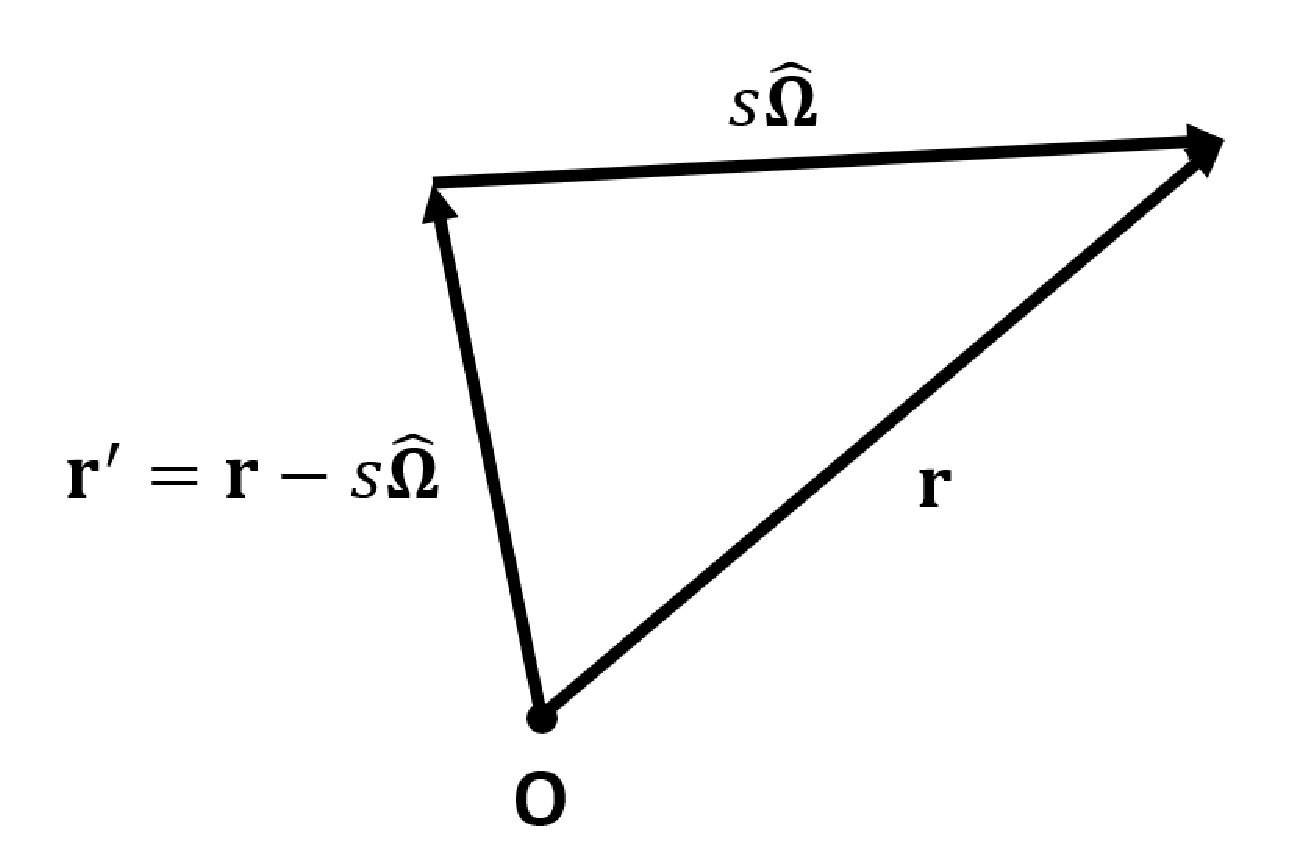
\includegraphics[width=80mm]{figure/path-s.eps}
  \caption{座標$\mathbf{r}'$の図示}\label{path-s}
  \end{center}
\end{figure}
\begin{equation}
  \mathbf{r}' = \mathbf{r} - s\SpcAng, \quad t' = t - \frac{s}{v}
\end{equation}
である。あるスカラーの関数$f(\mathbf{r}', t')$について、
$\mathbf{r}'(s), t'(s)$の合成関数と見れば、今表現したい微分は
\begin{align}
  \frac{df}{ds}
  \ = \frac{\partial f}{\partial \mathbf{r}'} \frac{\partial \mathbf{r}'}{\partial s} + \frac{\partial f}{\partial t'} \frac{\partial t'}{\partial s}
  \ = \frac{\partial f}{\partial \mathbf{r}'} \cdot (-\SpcAng) + \frac{\partial f}{\partial t'} (-\frac{1}{v})
  \ = -\SpcAng \cdot \nabla' f - \frac{1}{v} \frac{\partial f}{\partial t'}
\end{align}
角度中性子束$\psi$についてこの微分を考えれば、中性子が飛行している方向に沿って移動しながら、
角度束がどう変わっていくかを示す微分となる。そして、中性子輸送方程式の
漏洩率と時間変化部分はこの微分で置き換えられることが分かる。
よって、座標を$(\mathbf{r}', t')$に置き換えた中性子輸送方程式~\eqref{trans-Q}は
\begin{equation}
  \left( \frac{d}{ds} - \Sigma_t(\mathbf{r} - s\SpcAng, E) \right) \psi(\mathbf{r} - s\SpcAng, E, \SpcAng, t - s/v) = 
  -Q(\mathbf{r} - s\SpcAng, E, \SpcAng, t - s/v) \label{trans-s}
\end{equation}
となる。この微分方程式は

\begin{equation}
  \frac{df(s)}{ds} + P(s)f(s) = Q(s)
\end{equation}

の形をしている非斉次一階線形微分方程式で、積分因子法を用いて解くことができる。
積分因子法は

\begin{equation}
  g(s) \left( \frac{df(s)}{ds} + P(s)f(s) \right) = \frac{d}{ds} \left( g(s) f(s) \right) \label{Int-factor}
\end{equation}

となるように積分因子$g(s)$を決めれば、
\begin{equation}
  \frac{d}{ds} \left( g(s) f(s) \right) = g(s) Q(s)
\end{equation}
となり、積分により$g(s)f(s)$が求まるという解法である。
積分因子の条件~\eqref{Int-factor}より、

\begin{align}
  &\text{左辺は} \quad g(s) \left( \frac{df}{ds} + P(s) f \right) = g(s) \frac{df}{ds} + g(s) P(s) f \notag\\
  &\text{右辺は} \quad \frac{d}{ds} \left( g(s) f(s) \right) = g(s) \frac{df}{ds} + \frac{dg}{ds} f \notag \\
\end{align}

両辺を見比べると$g(s) \frac{df}{ds}$が削除出来て、積分因子は

\begin{equation}
  \frac{dg}{ds} = g(s) P(s)
\end{equation}

を満たさなければならない。
したがって、式~\eqref{trans-s}の積分因子は
\begin{align}
  \frac{dg}{ds} &= -\Sigma_t(\mathbf{r} - s\SpcAng, E) g(s) \notag \\
  \frac{dg}{g} &= -\Sigma_t(\mathbf{r} - s\SpcAng, E) \ ds \notag \\
  \int_{0}^{s} \frac{1}{g} \frac{dg}{ds} \ ds &= \int_{0}^{s} -\Sigma_t(\mathbf{r} - s\SpcAng, E,E) \ ds' \notag \\
  \ln{g(s)} - \ln{g(0)} &= - \int_{0}^{s} \Sigma_t(\mathbf{r} - s'\SpcAng, E) \ ds' \notag \\
  \text{$g(0)=1$として} \quad g(s) &= \mathrm{exp} \left( - \int_{0}^{s} \Sigma_t(\mathbf{r} - s'\SpcAng, E) \ ds' \right) \label{trans-Int-factor}
\end{align}
この積分因子を式~\eqref{trans-s}の両辺に掛けると

%\newcommand{\gs}{\mathrm{exp} \left( - \int_{0}^{s} \Sigma_t(\mathbf{r} - s'\SpcAng) \ ds' \right)}
%\newcommand{\gsd}{\mathrm{exp} \left( - \int_{0}^{s'} \Sigma_t(\mathbf{r} - s''\SpcAng) \ ds'' \right)}
\newcommand{\gs}{e^{ - \int_{0}^{s} \Sigma_t(\mathbf{r} - s'\SpcAng) \ ds' }}
\newcommand{\gsd}{e^{ - \int_{0}^{s'} \Sigma_t(\mathbf{r} - s''\SpcAng) \ ds'' }}
\newcommand{\rsO}{\mathbf{r} - s\SpcAng}
\newcommand{\rsdO}{\mathbf{r} - s'\SpcAng}
\newcommand{\tsv}{t - s/v}
\newcommand{\tsdv}{t - s'/v}
\begin{align}
  \frac{d}{ds} \left[ \gs \psi(\rsO, \tsv) \right] \notag\\
   = - \gs Q(\rsO, \tsv)
\end{align}
なお、表記の簡略化のためエネルギーと飛行方向の変数$E, \SpcAng$を省いた。
この式を$0 \rightarrow s$で積分すれば、角度束$\psi$についての式を得ることが出来る。
左辺について、
\begin{align}
  &\int_0^s \frac{d}{ds'} \left[ \gsd \psi(\rsdO, \tsdv) \right] \ ds' \notag \\
  &= \left[ \gsd \psi(\rsdO, \tsdv) \right]_0^s \notag \\
  &= \gs \psi(\rsO, \tsv) - \mathrm{exp}(0) \psi(\mathbf{r}, t)
\end{align}
なので、輸送方程式は
\begin{align}
  \psi(\rEOt) = e^{-\int_{0}^{s} \Sigma_t(\mathbf{r} - s'\SpcAng, E) \ ds'} \psi(\rsO, E, \SpcAng, \tsv) \notag \\
  + \int_0^s \left[ e^{-\int_{0}^{s'} \Sigma_t(\mathbf{r} - s''\SpcAng, E) \ ds''} Q(\rsdO, E, \SpcAng, \tsdv) \right] \ ds' \label{int-trans-pre}
\end{align}
となる。

この式の物理的意味は次のように説明できる。
右辺第1項は$s$だけ巻き戻された$\SpcAng$方向の角度束に、位置$\mathbf{r}$まで衝突せずに
進む確率$\gs$を掛けたものである。右辺第2項の被積分関数は、線源または散乱によって生成される
$s'$だけ巻き戻された位置、時刻の中性子数に$s'$の距離を衝突せずに進む確率$\gsd$を掛けたもの
である。これを$0$から$s$まで積分したものが右辺第2項となる。

この式を導出する際の積分範囲を$s \rightarrow \infty$とすると右辺第1項が消えて、
積分型中性子輸送方程式となる。
\vskip.5\baselineskip
\begin{itembox}[l]{積分型中性子輸送方程式}
  \begin{equation}
    \psi(\rEOt) 
    = \int_{0}^{\infty} e^{ - \int_{0}^{s} \Sigma_t(\mathbf{r} - s'\SpcAng, E) \ ds'} Q(\rsO, E, \SpcAng, \tsv) \ ds \label{int-trans}
  \end{equation}
  ただし、$Q(\rsO, E, \SpcAng, \tsv)$は
  \begin{align}
    &Q(\rsO, E, \SpcAng, \tsv) = \notag \\
    &\int_{4 \pi} \int_{0}^{\infty} \left[  
    \Sigma_s (\rsO, \EOtoEO) \psi(\rsO, E', \SpcAng', \tsv) \right] dE' d\SpcAng' \notag\\
    &+ s(\rsO, E, \SpcAng, \tsv)
  \end{align}
\end{itembox}
\vskip.5\baselineskip
これは微積分型輸送方程式~\eqref{transport}に、無限遠で角度束が$0$となる境界条件を
あたえたものと等価である。
式~\eqref{int-trans-pre}と~\eqref{int-trans}は共に格子体系の中性子束計算によく使われる。

\newpage

\subsection{中性子拡散方程式}
原子炉物理の計算で多くの場合必要になるのが核反応率$\Sigma \phi$であるため、
角度中性子束を角度で積分して中性子束の方程式を得たい。そこで、近似を導入し
輸送方程式を中性子束の方程式に変形する。






% 章ごとの参考文献欄
\printbibliography[segment=\therefsegment,heading=subbibliography]

\newpage

%\include{}



\end{document}